%===============================================================================
% LaTeX sjabloon voor de bachelorproef toegepaste informatica aan HOGENT
% Meer info op https://github.com/HoGentTIN/latex-hogent-report
%===============================================================================

\documentclass[dutch,dit,thesis]{hogentreport}

% TODO:
% - If necessary, replace the option `dit`' with your own department!
%   Valid entries are dbo, dbt, dgz, dit, dlo, dog, dsa, soa
% - If you write your thesis in English (remark: only possible after getting
%   explicit approval!), remove the option "dutch," or replace with "english".

\usepackage{lipsum} % For blind text, can be removed after adding actual content

%% Pictures to include in the text can be put in the graphics/ folder
\graphicspath{{graphics/}}

%% For source code highlighting, requires pygments to be installed
%% Compile with the -shell-escape flag!
%% \usepackage[section]{minted}
%% If you compile with the make_thesis.{bat,sh} script, use the following
%% import instead:
\usepackage[section,outputdir=../output]{minted}
\usemintedstyle{solarized-light}
\definecolor{bg}{RGB}{253,246,227} %% Set the background color of the codeframe

%% Change this line to edit the line numbering style:
\renewcommand{\theFancyVerbLine}{\ttfamily\scriptsize\arabic{FancyVerbLine}}

%% Macro definition to load external java source files with \javacode{filename}:
\newmintedfile[javacode]{java}{
    bgcolor=bg,
    fontfamily=tt,
    linenos=true,
    numberblanklines=true,
    numbersep=5pt,
    gobble=0,
    framesep=2mm,
    funcnamehighlighting=true,
    tabsize=4,
    obeytabs=false,
    breaklines=true,
    mathescape=false
    samepage=false,
    showspaces=false,
    showtabs =false,
    texcl=false,
}

% Other packages not already included can be imported here

%%---------- Document metadata -------------------------------------------------
% TODO: Replace this with your own information
\author{Quinten De Wolf}
\supervisor{Mevr M. Van Audenrode}
\cosupervisor{Mr. D. Van Der Elst}
\title[]%
    {De beste JavaScript runtime-omgeving voor performante applicaties: een vergelijkende studie}
\academicyear{\advance\year by -1 \the\year--\advance\year by 1 \the\year}
\examperiod{1}
\degreesought{\IfLanguageName{dutch}{Professionele bachelor in de toegepaste informatica}{Bachelor of applied computer science}}
\partialthesis{false} %% To display 'in partial fulfilment'
%\institution{Internshipcompany BVBA.}

%% Add global exceptions to the hyphenation here
\hyphenation{back-slash}

%% The bibliography (style and settings are  found in hogentthesis.cls)
\addbibresource{bachproef.bib}            %% Bibliography file
\addbibresource{../voorstel/voorstel.bib} %% Bibliography research proposal
\defbibheading{bibempty}{}

%% Prevent empty pages for right-handed chapter starts in twoside mode
\renewcommand{\cleardoublepage}{\clearpage}

\renewcommand{\arraystretch}{1.2}

%% Content starts here.
\begin{document}

%---------- Front matter -------------------------------------------------------

\frontmatter

\hypersetup{pageanchor=false} %% Disable page numbering references
%% Render a Dutch outer title page if the main language is English
\IfLanguageName{english}{%
    %% If necessary, information can be changed here
    \degreesought{Professionele Bachelor toegepaste informatica}%
    \begin{otherlanguage}{dutch}%
       \maketitle%
    \end{otherlanguage}%
}{}

%% Generates title page content
\maketitle
\hypersetup{pageanchor=true}

%%=============================================================================
%% Voorwoord
%%=============================================================================

\chapter*{\IfLanguageName{dutch}{Woord vooraf}{Preface}}%
\label{ch:voorwoord}

%% TODO:
%% Het voorwoord is het enige deel van de bachelorproef waar je vanuit je
%% eigen standpunt (``ik-vorm'') mag schrijven. Je kan hier bv. motiveren
%% waarom jij het onderwerp wil bespreken.
%% Vergeet ook niet te bedanken wie je geholpen/gesteund/... heeft

Met trots presenteer ik mijn bachelorproef "De beste JavaScript runtime-omgeving voor performante applicaties: een vergelijkende studie", 
waarin ik, in het kader voor het voltooien van mijn opleiding Toegepaste Informatica, Node.js vergelijk met het opkomende Bun op vlak van performantie.
Tijdens mijn studiejaren ben ik altijd geïnteresseerd geweest in JavaScript runtime-omgevingen zoals onder andere Node.js en Bun en
hoe deze tegen over elkaar staan. Toen ik een onderwerp moest kiezen kwam dit direct in me op aangezien het mij interessant leek om me dieper te verdiepen 
in Bun. Het schrijven van deze bachelorproef heeft me dan ook uitgedaagd om mijn kennis en vaardigheden te verbreden.
\vspace{5mm}
Ik wil mijn oprechte dank betuigen aan iedereen die heeft bijgedragen aan deze bachelorproef, 
in het bijzonder mijn promotor Mevr M. Van Audenrode en mijn co-promotor Mr. D. Van Der Elst voor hun
waardevolle begeleiding en feedback gedurende het hele proces. 
Zij stonden altijd klaar voor vragen en gaven telkens constructieve en gerichte feedback waarvoor ik hun zeer dankbaar ben.
\vspace{5mm}

Tot slot wil ik mijn ouders bedanken voor de kansen die zij mij hebben gegeven. 
Dankzij hun dagelijkse inzet kan ik mij telkens concentreren op mijn studies.



%%=============================================================================
%% Samenvatting
%%=============================================================================

% TODO: De "abstract" of samenvatting is een kernachtige (~ 1 blz. voor een
% thesis) synthese van het document.
%
% Een goede abstract biedt een kernachtig antwoord op volgende vragen:
%
% 1. Waarover gaat de bachelorproef?
% 2. Waarom heb je er over geschreven?
% 3. Hoe heb je het onderzoek uitgevoerd?
% 4. Wat waren de resultaten? Wat blijkt uit je onderzoek?
% 5. Wat betekenen je resultaten? Wat is de relevantie voor het werkveld?
%
% Daarom bestaat een abstract uit volgende componenten:
%
% - inleiding + kaderen thema
% - probleemstelling
% - (centrale) onderzoeksvraag
% - onderzoeksdoelstelling
% - methodologie
% - resultaten (beperk tot de belangrijkste, relevant voor de onderzoeksvraag)
% - conclusies, aanbevelingen, beperkingen
%
% LET OP! Een samenvatting is GEEN voorwoord!

%%---------- Nederlandse samenvatting -----------------------------------------
%
% TODO: Als je je bachelorproef in het Engels schrijft, moet je eerst een
% Nederlandse samenvatting invoegen. Haal daarvoor onderstaande code uit
% commentaar.
% Wie zijn bachelorproef in het Nederlands schrijft, kan dit negeren, de inhoud
% wordt niet in het document ingevoegd.

\IfLanguageName{english}{%
\selectlanguage{dutch}
\chapter*{Samenvatting}
\lipsum[1-4]
\selectlanguage{english}
}{}

%%---------- Samenvatting -----------------------------------------------------
% De samenvatting in de hoofdtaal van het document

\chapter*{\IfLanguageName{dutch}{Samenvatting}{Abstract}}

Performantie is doorheen de tijd alsmaar belangrijker geworden. 
Een goed presterende applicatie draagt bij aan een betere gebruikerservaring.
Gedurende deze tijd zijn er voortdurend nieuwe JavaScript runtime-omgevingen ontwikkeld met telkens nieuwe verbeteringen om
zo de noden van de alsmaar complexere applicaties te vervullen. 
Ondanks deze nieuwe ontwikkelingen worden weinig ervan effectief in de praktijk gebruikt.
Zo wordt het oudere Node.js vaak nog gekozen als JavaScript runtime-omgeving bij de ontwikkeling van applicaties.
Dit onderzoek heeft als doel inzicht te verschaffen in de performantie van Node.js en één van deze nieuwe omgevingen
om zo een correcte keuze te kunnen maken bij de ontwikkeling van performante applicaties.
De onderzoeksvraag hierbij is of één van deze nieuwe frameworks  
een correcte plaatsvervanger kan zijn voor Node.js bij de ontwikkeling van applicaties binnen bedrijven 
waar performantie centraal staat. Het onderzoek kan dan gebruikt worden als basis 
voor het maken van een doordachte backend keuze.
Om een antwoord te bekomen werd eerst informatie over het onderzoeksdomein verzameld om zo een duidelijk beeld ervan te schetsen.
Hierbij werden in de literatuurstudie Javascript runtime-omgevingen zoals Node.js, Deno en Bun besproken.
Nadien wordt aan de hand van een requirements-analyse één omgeving geselecteerd die het meest geschikt is als potentiële plaatsvervanger voor Node.js.
Hierbij voldeed Bun aan alle requirements en werd er gekozen om deze omgeving te vergelijken met Node.js in de proof-of-concepts.
Aan de hand van het Quick Sort algoritme werd de performantie bij computationele berekeningen gemeten.
Daarnaast werd ook een applicatie opgesteld met de mogelijkheid om data op te halen en in te voegen. 
Hierbij werd de performantie van beide omgevingen gemeten bij het afhandelen van netwerkverzoeken.
Dezelfde applicatie werd ook gebruikt om de installatietijd van de respectievelijke package managers te meten.
Hierbij heeft Bun een snellere installatietijd dan Node.js.
Bij het meten van het Quick Sort algoritme heeft Bun ook een snellere uitvoeringstijd wat het standpunt 
ondersteunt dat Bun beter presteert bij het uitvoeren van computationele berekeningen.
Tot slot heeft Bun een lagere latentie en een betere verwerking van het aantal verzoeken per seconde bij het ophalen en
invoegen van data ten koste van het CPU-gebruik en geheugengebruik.
Dit leidt tot de conclusie dat Bun een optimale keuze kan zijn voor applicaties met complexe algoritmes en calculaties. Echter, 
bij applicaties waarbij I/O-taken worden uitgevoerd, moet telkens een afweging gemaakt worden tussen de snellere verwerking van Bun
en het hogere middelengebruik dathiermee gepaard gaat.




%---------- Inhoud, lijst figuren, ... -----------------------------------------

\tableofcontents

% In a list of figures, the complete caption will be included. To prevent this,
% ALWAYS add a short description in the caption!
%
%  \caption[short description]{elaborate description}
%
% If you do, only the short description will be used in the list of figures

\listoffigures

% If you included tables and/or source code listings, uncomment the appropriate
% lines.
\listoftables
\listoflistings

% Als je een lijst van afkortingen of termen wil toevoegen, dan hoort die
% hier thuis. Gebruik bijvoorbeeld de ``glossaries'' package.
% https://www.overleaf.com/learn/latex/Glossaries

%---------- Kern ---------------------------------------------------------------

\mainmatter{}

% De eerste hoofdstukken van een bachelorproef zijn meestal een inleiding op
% het onderwerp, literatuurstudie en verantwoording methodologie.
% Aarzel niet om een meer beschrijvende titel aan deze hoofdstukken te geven of
% om bijvoorbeeld de inleiding en/of stand van zaken over meerdere hoofdstukken
% te verspreiden!

%%=============================================================================
%% Inleiding
%%=============================================================================

\chapter{\IfLanguageName{dutch}{Inleiding}{Introduction}}%
\label{ch:inleiding}


Door de jaren heen zijn applicaties alsmaar complexer geworden. Hierbij worden vaak achterliggend netwerkverzoeken afgehandeld door een 
een backend applicatie. Deze applicatie draait in een runtime-omgeving buiten de browser, 
waardoor deze toegang heeft tot databanken en netwerken van de server waarop het wordt uitgevoerd.
Een manier om zo een backend te ontwikkelen is met behulp van de programmeertaal JavaScript. 
Backend JavaScript applicaties worden dan uitgevoerd in een JavaScript runtime omgeving.
De meest populaire omgeving is Node.js. Zo toont onderzoek van ~\textcite{Greif2022} aan dat 93.6\% van de 29888 bevraagden Node.js 
regulier gebruiken.
Dit tegenover de 11.2\% en 4.3\% van de mensen die andere omgevingen zoals respectievelijk Deno en Bun gebruiken.
Deze 2 omgevingen zijn relatief jonger dan Node.js.

\section{\IfLanguageName{dutch}{Probleemstelling}{Problem Statement}}%
\label{sec:probleemstelling}

Performantie is doorheen de tijd alsmaar belangrijker geworden. 
Een performante applicatie zorgt hierbij voor een betere gebruikerservaring. 
Momenteel blijft Node.js de standaard keuze voor veel projecten. Niettemin zijn er nog tal van andere JavaScript runtime-omgevingen
, zoals Bun en Deno, die in staat zijn om de specifieke noden te vervullen waar Node.js niet aan kan voldoen. In dit onderzoek wordt geprobeerd 
een inzicht te verschaffen in de performantie van Node.js en één van deze nieuwe omgevingen,
om zo een weloverwogen keuze te kunnen maken bij de ontwikkeling van performante applicaties.
Dit onderzoek is relevant voor bedrijven waar performantie een essentiële rol speelt binnen de ontwikkeling van JavaScript backend applicaties en kan dienen als basis 
voor het maken van een doordachte backend keuze. Dit onderzoek 
biedt ook inzicht in de capaciteiten van Bun voor andere betrokkenen binnen het vakgebied van JavaScript backend ontwikkeling.

\section{\IfLanguageName{dutch}{Onderzoeksvraag}{Research question}}%
\label{sec:onderzoeksvraag}

In dit onderzoek wordt bestudeerd of één van deze nieuwe omgevingen
een correcte plaatsvervanger kan zijn voor Node.js bij de ontwikkeling van performante applicaties binnen bedrijven 
waar een JavaScript runtime wordt gebruikt.
Hierbij spelen verschillende aspecten een rol die aan de hand van volgende deelvragen worden onderzocht:
\begin{itemize}
  \item Wat zijn de onderliggende verschillen tussen Node.js en de andere omgeving?
  \item Is de gekozen omgeving performanter dan Node.js bij het uitvoeren van computationele berekeningen?
  \item Is de gekozen omgeving performanter dan Node.js bij het afhandelen van netwerkverzoeken?
  \item Wat is het verschil tussen hun respectievelijke package managers?
\end{itemize}

\section{\IfLanguageName{dutch}{Onderzoeksdoelstelling}{Research objective}}%
\label{sec:onderzoeksdoelstelling}

Dit onderzoek heeft als doel inzicht te verschaffen in de performantie van Node.js en één van deze nieuwe omgevingen
om zo een correcte keuze te kunnen maken bij de ontwikkeling van performante applicaties. Dit wordt bereikt door middel van een vergelijkende studie
waarbij zowel de geselecteerde omgeving als Node.js worden getest aan de hand proof-of-concepts. 
Hierbij worden de prestaties gemeten tijdens computationele berekeningen en het afhandelen van netwerkverzoeken, waarbij specifiek gekeken wordt naar
de latentie, aantal verzoeken per seconde, installatietijd en uitvoeringstijd. 
Het doel is deze resultaten te gebruiken om vast te stellen of de gekozen omgeving performanter is dan Node.js. 
Het onderzoek wordt als succesvol beschouwd als er aan de hand van deze resultaten een duidelijk verschil tussen de omgevingen zichtbaar is.
\section{\IfLanguageName{dutch}{Opzet van deze bachelorproef}{Structure of this bachelor thesis}}%
\label{sec:opzet-bachelorproef}

% Het is gebruikelijk aan het einde van de inleiding een overzicht te
% geven van de opbouw van de rest van de tekst. Deze sectie bevat al een aanzet
% die je kan aanvullen/aanpassen in functie van je eigen tekst.

De rest van deze bachelorproef is als volgt opgebouwd:

In hoofdstuk~\ref{ch:stand-van-zaken} wordt een overzicht gegeven van de stand van zaken binnen het onderzoeksdomein,
 op basis van een literatuurstudie.

In hoofdstuk~\ref{ch:methodologie} wordt de methodologie toegelicht en worden de gebruikte onderzoekstechnieken besproken om een antwoord te kunnen formuleren 
op de onderzoeksvragen.

In hoofdstuk~\ref{ch:selectie} wordt de lijst van omgevingen afgetoetst aan de opgegegeven requirements om uiteindelijk een geschikte omgeving te selecteren.

In hoofdstuk~\ref{ch:proof-of-concept} wordt de opzet en metingen van de proof-of-concepts toegelicht. Op het einde worden de bekomen resultaten besproken.

In hoofdstuk~\ref{ch:conclusie}, tenslotte, 
wordt de conclusie gegeven en een antwoord geformuleerd op de onderzoeksvragen. 
Daarbij wordt ook een aanzet gegeven voor toekomstig onderzoek binnen dit domein.
\chapter{\IfLanguageName{dutch}{Stand van zaken}{State of the art}}%
\label{ch:stand-van-zaken}

% Tip: Begin elk hoofdstuk met een paragraaf inleiding die beschrijft hoe
% dit hoofdstuk past binnen het geheel van de bachelorproef. Geef in het
% bijzonder aan wat de link is met het vorige en volgende hoofdstuk.

% Pas na deze inleidende paragraaf komt de eerste sectiehoofding.

Dit hoofdstuk bevat je literatuurstudie. 
De inhoud gaat verder op de inleiding, maar zal het onderwerp van de bachelorproef *diepgaand* uitspitten. 
De bedoeling is dat de lezer na lezing van dit hoofdstuk helemaal op de hoogte is van de huidige stand van zaken (state-of-the-art) 
in het onderzoeksdomein. 
Iemand die niet vertrouwd is met het onderwerp, 
weet nu voldoende om de rest van het verhaal te kunnen volgen, 
zonder dat die er nog andere informatie moet over opzoeken \autocite{Pollefliet2011}.

Je verwijst bij elke bewering die je doet, vakterm die je introduceert, enz.\ naar je bronnen. 
In \LaTeX{} kan dat met het commando \texttt{$\backslash${textcite\{\}}} of \texttt{$\backslash${autocite\{\}}}. 
Als argument van het commando geef je de ``sleutel'' van een ``record'' in een bibliografische databank in het Bib\LaTeX{}-formaat
 (een tekstbestand). Als je expliciet naar de auteur verwijst in de zin (narratieve referentie), 
 gebruik je \texttt{$\backslash${}textcite\{\}}. Soms is de auteursnaam niet expliciet een onderdeel van de zin, 
 dan gebruik je \texttt{$\backslash${}autocite\{\}} (referentie tussen haakjes). Dit gebruik je bv.~bij een citaat, 
 of om in het bijschrift van een overgenomen afbeelding, broncode, tabel, enz. te verwijzen naar de bron. 
 In de volgende paragraaf een voorbeeld van elk.

\textcite{Knuth1998} schreef een van de standaardwerken over sorteer- en zoekalgoritmen. 
Experten zijn het erover eens dat cloud computing een interessante opportuniteit vormen, zowel voor gebruikers als voor dienstverleners op vlak van informatietechnologie~\autocite{Creeger2009}.

Let er ook op: het \texttt{cite}-commando voor de punt, dus binnen de zin. Je verwijst meteen naar een bron in de eerste zin die erop gebaseerd is, 
dus niet pas op het einde van een paragraaf.



Dit hoofdstuk bevat een literatuurstudie die de gebruikten technologieën gaat omschrijven. 
Daarnaast worden ook eerdere studies naar deze technologieën vermeld. 
Ten eerste wordt een precieze beschrijving gegeven over de programmeertaal javascript en hoe deze wordt gebruikt bij de runtime-omgevingen.
Nadien wordt verder ingegaan op 2 van deze omgevingen namelijk Node.js en Bun.

\section{Javascript}
Javascript is een programmeertaal die gebruikt wordt om applicaties te ontwikkelen. 
Specifiek is het een scripting taal die gebruikt om web pagina's interactief te maken~\autocite{Mozilla2023}.
Hierbij spreken we over client-side Javascript. Wanneer een web pagina wordt bekeken zal de javascript code worden 
gedownload en uitgevoerd~\autocite{JonathanBrownCFA2024}. Langs de andere kant heb je ook nog Server-side javascript. 
Hierbij wordt de code uitgevoerd op de server in plaats van op de client~\autocite{JonathanBrownCFA2024}. 
Voor deze code dan te laten uitvoeren is een javascript runtime-omgeving nodig. 

\subsection{Javascript runtime-omgeving}
Een javascript-omgeving bestaat uit alle componenten om javascript correct te laten werken ~\autocite{Christopher}. 
Het bevat een JavaScript engine, WEB APIs en een callback queue ~\autocite{Christopher}. 
Deze runtime zal dan javascript code omzetten in code die verstaanbaar is voor de computer.
De omgeving specificeert waar dit wordt gedaan, dit kan in een browser maar ook in andere omgevingen zoals een server.
Met behulp van javascript runtime-omgevingen zoals Node.js en Bun kan javascript code ook buiten de browser worden uitgevoerd~\autocite{Mozilla2023}.

\subsubsection{Javascript engine, WEB APIs en callback queue}

In een artikel van ~\textcite{Christopher}, 
wordt uitgelegd dat de javascript engine een simpel computer programma is dat de code kan interpreteren en uitvoeren.
Elk browser heeft zijn eigen Javascript engine achterliggend. Het meest bekende hiervan is de
V8 engine die zowel bij Google chrome als Node.js wordt gebruikt. 
Wanneer een stuk code in de engine wordt gestoken zal deze eerst gelezen worden (parsing). 
De code wordt hierbij omgezet in een data structuur genaamd abstract syntax tree (AST).
Wanneer deze boom is aangemaakt zal de compiler deze omzetten naar machine code. 
Eenmaal deze code is gegenereerd zal de engine zogenaamde execution contexts aanmaken om de code uit te voeren.
In figuur ~\ref{fig:javascriptengine} wordt hiervan een visuele voorstelling getoond.
\begin{figure}[H]
    \centering
    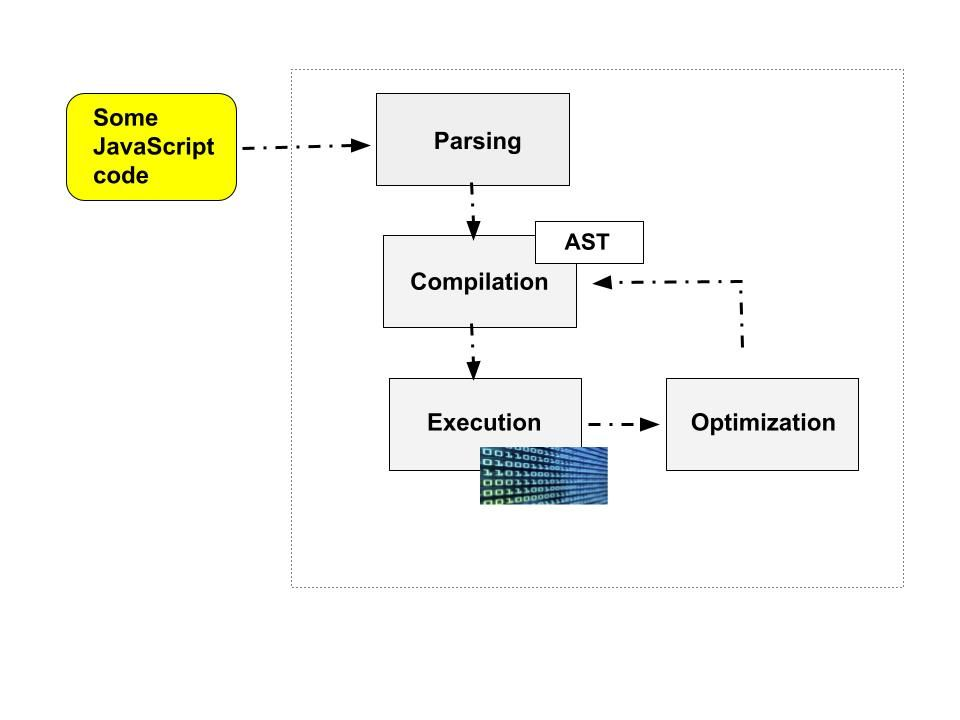
\includegraphics[width=.9\textwidth]{graphics/javascriptengine.jpeg}
    \caption{\label{fig:javascriptengine}}Visuele voorstelling van werking javascript engine ~\autocite{Christopher}.
\end{figure}

Naast een Javascript engine bevat een runtime-omgeving ook WEB APIs en een callback queue. 
WEB APIs zijn functionaliteiten die specifiek voor de runtime omgeving zijn en dus geen deel uitmaken van de javascript taal.
De callback queue zorgt ervoor dat callback functions volgens de First-In-First-Out methode worden uitgevoerd.

\section{Node.js}
De afgelopen jaren is het aantal runtime-omgevingen sterk toegenomen. De meest bekende en oudste hiervan is Node.js.
Node.js is een server-side framework dat wordt gebruikt voor schaalbare applicaties te maken ~\autocite{Gackenheimer2013}.
Het maakt gebruik van de javascript V8 engine ontwikkeld door Google en heeft zijn eigen package manager genaamd Node Package Manager (npm).

\subsection{Event loop}
In het boek van ~\textcite{Ali2013} wordt verteld hoe Node.js zich onderscheidt van andere platformen door het gebruik van een event loop.
Wanneer in Node.js data wordt gelezen of geschreven zal een gebeurtenis worden uitgezonden. 
Aan de hand van zelfgedefinieerde callbacks, verwijzingen naar uitvoerbare code, kan gereageerd worden op deze gebeurtenissen. 
De event loop zal hierbij continu kijken of er gebeurtenissen voorkomen, en wanneer dit zo is zal het deze in de event wachtrij plaatsen.
De event loop zal dan deze wachtrij doorgaan en één per één de event handlers uitvoeren. 
Dit laat toe om I/O operaties asynchroon te maken zonder hierbij multithreading te gebruiken.
In figuur ~\ref{fig:eventloop} wordt hiervan een visuele voorstelling getoond.
\begin{figure}[h]
    \centering
    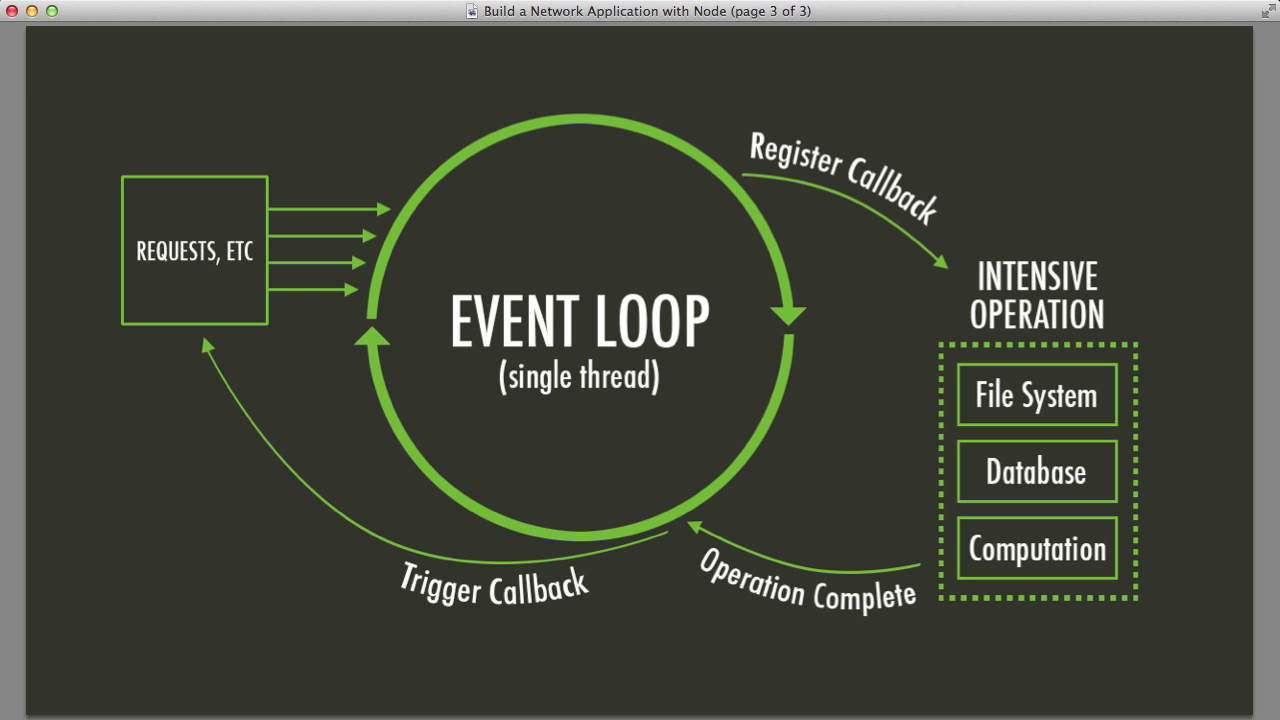
\includegraphics[width=.9\textwidth]{graphics/eventloop.png}
    \caption{\label{fig:eventloop}}Visuele voorstelling van de event loop ~\autocite{Luxembourg2023}.
\end{figure}

\subsection{Node Package Manager}
Node.js maakt gebruik van modules om code te hergebruiken. 
Zo vormt een module een stuk herbruikbare javascript code 
die je kan importeren in een ander javascript bestand ~\autocite{Semah2022}.
Naast deze zelf te maken kan je ook modules of packages van andere ontwikkelaars gebruiken met behulp van de Node Package Manager.
Veel van deze packages hangen af van nog andere packages om correct te werken \autocite{kula2017}.
Aan de hand van een package.json bestand kunnen packages toegevoegd worden aan een project.
\begin{figure}[h!]
    \centering
    \begin{minted}[bgcolor=bg,
        fontfamily=tt,
        linenos=true,
        numberblanklines=true,
        numbersep=5pt,
        gobble=0,
        framesep=2mm,
        tabsize=4,
        obeytabs=false,
        breaklines=true,
        mathescape=false
        samepage=false,
        showspaces=false,
        showtabs =false,
        texcl=false]{js}
        {
          "dependencies": {
            "foo": "1.0.0 - 2.9999.9999",
            "bar": ">=1.0.2 <2.1.2",
            "baz": ">1.0.2 <=2.3.4",
            "boo": "2.0.1",
            "qux": "<1.0.0 || >=2.3.1 <2.4.5 || >=2.5.2 <3.0.0",
            "asd": "http://asdf.com/asdf.tar.gz",
            "til": "~1.2",
            "elf": "~1.2.3",
            "two": "2.x",
            "thr": "3.3.x",
            "lat": "latest",
            "dyl": "file:../dyl"
            }
        }
        \end{minted}
        \caption{Voorbeeld package.json \autocite{Kaplan2024}}
\end{figure}

\section{Bun}
Performantie is één van de belangrijkste zaken bij een server-side framework. 
Daarom is Node.js dankzij zijn event-gedreven I/O model een veelvoorkomende keuze als het gaat om server-side frameworks.
Echter wil Bun dit veranderen door nog meer focus te leggen op snelheid en performantie.

\subsection{JavascriptCore}
Eén van de manieren waardoor Bun dit bereikt is door het gebruiken van een andere Javascript engine.
Bun gebruikt JavaScriptCore in plaats van de V8 Javascript engine die Node.js gebruikt. 
Deze zou volgens ~\textcite{McDonnel2023} ervoor zorgen dat Bun 4 keer sneller opstart dan Node.js. 
De engine is ingebouwd in WebKit, een web browser engine die wordt gebruikt binnen het Apple ecosysteem voor macOS en IOS.
In een artikel van ~\textcite{Pizlo2020} wordt uitgelegd dat bij de executie een script door verschillende fases gaat:
\begin{itemize}
    \item De lexer is verantwoordelijking voor het opbreken van het script in een reeks tokens.
    \item De parser gaat deze tokens gebruiken om een een asbract syntax tree te maken.
    \item De Low-Level Interpreter (LLINT) zal bytecode produceren dat JavaScriptCore kan uitvoeren.
\end{itemize}
Daarnaast zijn er hierbij ook nog optimalisaties voor instructies die vaak terugkeren. 
JavascriptCore zal instructies in 4 verschillende lagen uitvoeren, afhankelijk van hoeveel keer ze worden uitgevoerd:
\begin{enumerate}
    \item De Low-Level Interpreter (LLINT) zal zoals hierboven beschreven instructies omzetten in bytecode.
    \item De baseline JIT zal een stuk code at runtime uitvoeren in plaats van ervoor. 
    Hierbij worden de bytecode operaties omgezet naar een template van machine code zonder veel optimalisaties. Deze laag is snel.
    \item De Data Flow Graph JIT zal een data-flow graaf gebruiken van de code om zo complexe optimalisaties uit te voeren die betrekking hebben tot de stroom van de code.
    \item De Faster than Light JIT zal nog meer optimalisaties toevoegen bovenop de optimalisaties van de Data Flowh Graph JIT. 
    Deze laag is duurder en wordt enkel gebruikt voor code die kunnen profiteren van optimalisaties.
\end{enumerate}
Via de Low-Level Interpreter zal een profile voor elke instructie aangemaakt worden. 
Aan de hand hiervan weet de engine hoeveel keer een instructie wordt uitgevoerd en in welk niveau ze zitten.
LLINT zorgt ervoor dat het geheugengebruik wordt gereduceerd. Zo kost het genereren van machine code zeer veel geheugen.
Doormiddel van LLINT moeten we niet voor alle javascript code de bijhorende machine code genereren.
%%=============================================================================
%% Methodologie
%%=============================================================================

\chapter{\IfLanguageName{dutch}{Methodologie}{Methodology}}%
\label{ch:methodologie}

%% TODO: In dit hoofstuk geef je een korte toelichting over hoe je te werk bent
%% gegaan. Verdeel je onderzoek in grote fasen, en licht in elke fase toe wat
%% de doelstelling was, welke deliverables daar uit gekomen zijn, en welke
%% onderzoeksmethoden je daarbij toegepast hebt. Verantwoord waarom je
%% op deze manier te werk gegaan bent.
%% 
%% Voorbeelden van zulke fasen zijn: literatuurstudie, opstellen van een
%% requirements-analyse, opstellen long-list (bij vergelijkende studie),
%% selectie van geschikte tools (bij vergelijkende studie, "short-list"),
%% opzetten testopstelling/PoC, uitvoeren testen en verzamelen
%% van resultaten, analyse van resultaten, ...
%%
%% !!!!! LET OP !!!!!
%%
%% Het is uitdrukkelijk NIET de bedoeling dat je het grootste deel van de corpus
%% van je bachelorproef in dit hoofstuk verwerkt! Dit hoofdstuk is eerder een
%% kort overzicht van je plan van aanpak.
%%
%% Maak voor elke fase (behalve het literatuuronderzoek) een NIEUW HOOFDSTUK aan
%% en geef het een gepaste titel.

Het onderzoek bevat 4 fasen. 
De eerste fase bestaat uit het verzamelen van informatie over het onderzoeksdomein om zo een duidelijk beeld ervan te schetsen.
Dit wordt gedaan aan de hand van een literatuurstudie die te vinden is in hoofdstuk \ref{ch:stand-van-zaken}. 
Hierbij wordt eerst een algemene beschrijving over Javascript runtime-omgevingen besproken waarna 
er dieper wordt ingegaan op Node.js alsook zijn opvolger Deno en de nieuwe runtime Bun. 
Specifiek worden hun respectievelijke package managers, javascript engines, bundlers en extra functionaliteiten besproken.
Nadat er een duidelijker beeld is over het onderzoeksdomein wordt in de tweede fase, aan de hand van een requirements-analyse, 
één omgeving geselecteerd die het meest geschikt is als potentiële plaatsvervanger voor Node.js binnen de context van performante applicaties.
De requirements worden hier onderverdeeld via de MoSCoW-techniek in de categorieën “must-have”, “should-have”, “could-have” en “won't-have”. 
De alternatieven worden afgetoetst aan de requirements om zo tot één geschikte omgeving te komen die wordt vergeleken met Node.js.
In de derde fase worden zelfgemaakte proof-of-concepts opgesteld en getest (zie hoofdstuk \ref{ch:proof-of-concept}) voor beide omgevingen. 
Hierbij wordt een applicatie ontwikkeld waarbij een gebruiker onderwerpen kan ophalen en 
een recensie kan creëren over een bepaald onderwerp,
alsook een script dat een algoritme bevat. Hierdoor kunnen zowel metingen gedaan worden op computationele taken als I/O-taken (Input/Output).
De metingen worden uitgevoerd door 2 benchmark tools, Hyperfine en Bombardier, om volgende zaken te meten:
\begin{itemize}
    \item De latentie van de applicatie HTTP-verzoeken.
    \item Het aantal verzoeken per seconde bij de applicatie.
    \item De uitvoeringstijd van de berekeningen van het Quick Sort algoritme.
    \item Het geheugengebruik bij de applicatie.
    \item De installatietijd voor de respectievelijke package managers.
    \item Het CPU-gebruik bij de applicatie.
\end{itemize}
Daarnaast zal ook gekeken worden naar de extra functionaliteiten en hoe deze de complexiteit beïnvloeden.
Aan de hand van deze resultaten komen we tot de laatste fase namelijk de conclusie. 
Hierbij worden de data geanalyseerd om zo een antwoord te formuleren op de onderzoeksvragen.
Hieruit wordt afgeleid of het gekozen framework een geschikte plaatsvervanger kan zijn voor Node.js binnen 
de ontwikkeling van applicaties waar performantie centraal staat.

%%=============================================================================
%% Selectie
%%=============================================================================

\chapter{\IfLanguageName{dutch}{Selectie omgeving}{Selection environment}}%
\label{ch:selectie}

In dit hoofdstuk wordt aan de hand van een requirements-analyse een selectie gemaakt voor de JavaScript runtime omgeving 
die het meest geschikt zou zijn als potentiële plaatsvervanger van Node.js binnen de context van performante applicaties.
Er wordt gestart met een oplijsting van de requirements op basis van de MoSCoW-techniek in de categorieën “must-have”, “should-have” en “nice-to-have”. 
Daarna worden de alternatieven in de lijst afgetoetst aan deze requirements om zo tot één geschikte omgeving te komen die wordt vergeleken met Node.js.

\section*{Requirements}
In de volgende sectie wordt eerst uitgelegd wat MoSCoW betekent, 
waarna deze methode wordt toegepast om de verschillende requirements te bepalen.
\subsection{MoSCoW}
Voor de oplijsting van de requirements wordt gebruikgemaakt van de MoSCoW methode. 
In het boek van \textcite{Vliet2007} wordt uitgelegd wat deze methode precies inhoud. 
Zo dient MoSCoW om requirements te prioriteren. Het bestaat uit 4 lagen:
\begin{itemize}
    \item Must haves zijn requirements die zeker nodig zijn.
    \item Should haves zijn requirements die belangrijk zijn, maar niet absoluut nodig zijn voor een werkend systeem.
    \item Could haves zijn requirements die niet belangrijk zijn maar wel goed zijn om te hebben.
    \item Won't haves zijn requirements die niet nodig zijn.
\end{itemize}
In het onderzoek wordt deze methode toegepast om te weten waaraan een gepaste JavaScript omgeving moet voldoen.

\subsection{Must have requirements}
In volgende lijst zijn de requirements die zeker nodig zijn bij een JavaScript runtime-omgeving opgesomd:
\begin{itemize}
    \item De omgeving moet door een aanzienlijk aantal ontwikkelaars worden gebruikt.
    \item De omgeving moet goede prestaties bieden.
    \item De omgeving moet platformonafhankelijk zijn.
    \item De omgeving moet een modulesysteem bieden.
    \item Er moet een verscheidenheid aan bibliotheken en packages beschikbaar zijn voor de omgeving.
    \item De omgeving moet stabiel zijn en regelmatig updates ontvangen.
\end{itemize}
Aangezien dit onderzoek gebruikt kan worden als leidraad bij de keuze van een JavaScript runtime-omgeving, 
moet deze platformonafhankelijk zijn, wat inhoudt dat het op verschillende besturingssystemen kan worden gebruikt.
Het moet daarnaast ook door een aanzienlijk aantal ontwikkelaars worden gebruikt.
Dit wordt bepaald aan de hand van het jaarlijks onderzoek van \textcite{Greif2022} 
waarbij een minimumdrempel van 1\% van de respondenten wordt genomen.
Hierbij moet de omgeving ook stabiel en onderhouden zijn.
Daarnaast moet de omgeving een modulesyteem met een verscheidenheid aan bibliotheken bevatten 
zodat deze kan uitgebreid worden in functionaliteit. 
Als laatste moet de omgeving goede prestaties bieden bij zowel computationele berekeningen als I/O-taken
aangezien dit onderzoek zich focust op de performantie van de omgevingen.

\subsection{Should have requirements}
In volgende lijst zijn de requirements die belangrijk zijn bij een JavaScript runtime-omgeving opgesomd:
\begin{itemize}
    \item Er moet documentatie aanwezig zijn over de runtime-omgeving.
    \item De omgeving moet asynchrone I/O-operaties ondersteunen.
\end{itemize}
Voor de implementatie van de omgevingen is het belangrijk dat er voldoende documentatie aanwezig is.
Ook moeten deze asynchrone I/O-operaties ondersteunen zodat deze even performant of performanter kunnen werken als Node.js.

\subsection{Could have requirements}
In volgende lijst staan de requirements die “nice-to-have” zijn:
\begin{itemize}
    \item De omgeving heeft geïntegreerde ondersteuning voor TypeScript.
    \item De omgeving heeft een geïntegreerde test-runner.
    \item De omgeving heeft een geïntegreerde bundler.
\end{itemize}
Deze requirements zijn niet noodzakelijk maar kunnen behulpzaam zijn voor de gebruiker en de performantie van de runtime-omgeving.

\subsection{Won't have requirements}
In volgende lijst zijn de Won't have requirements:
\begin{itemize}
    \item De omgeving ondersteunt geen JavaScript.
    \item De omgeving laat geen benchmark testen toe. 
    \item De omgeving is closed-source.
\end{itemize}
De omgeving mag niet beschikken over deze requirements. 
Zo is het verplicht dat de omgeving een JavaScript runtime-omgeving is en dat deze benchmark testen mogelijk maakt om de prestaties te meten.
Daarnaast moet deze ook open-source zijn zodat er transparantie en onafhankelijkheid is.

\section{Selectie}
Nu dat de requirements bepaald zijn, worden de verschillende JavaScript runtime-omgevingen hier tegenover afgetoetst.
Deze lijst van runtime-omgevingen is gebaseerd op de samengestelde lijst van \textcite{Errilaz2023} 
zoals weergegeven in tabel \ref{tab:omgevingen}.
In tabel \ref{tab:requirements} worden deze omgevingen afgetoetst aan de requirements. 
Deze zal als basis dienen voor de selectie van een runtime-omgeving voor de vergelijking met Node.js.
\begin{table}[H]
    \begin{tabular}{|c|}
    \hline
    \textbf{Runtime omgevingen} \\ \hline
    Bun                         \\
    Deno                        \\
    Just                        \\
    Txiki.js                    \\
    Napa.js                     \\
    Elsa                        \\ \hline
    \end{tabular}
    \caption{\label{tab:omgevingen}Lijst van runtime omgevingen}
\end{table}


\begin{table}[]
    \begin{tabular}{|c|cccccc|}
    \hline
    \textbf{}                                                                                                                               & \multicolumn{6}{c|}{\textbf{Runtime omgevingen}}                                                                                                                       \\ \hline
    \textbf{Requirements}                                                                                                                   & \multicolumn{1}{l}{Bun} & \multicolumn{1}{l}{Deno} & \multicolumn{1}{l}{Just} & \multicolumn{1}{l}{Txiki.js} & \multicolumn{1}{l}{Napa.js} & \multicolumn{1}{l|}{Elsa} \\ \cline{1-1}
    \begin{tabular}[c]{@{}c@{}}De omgeving moet door\\ een aanzienlijk aantal ontwikkelaars\\ worden gebruikt\end{tabular}                  & x                       & x                        &                          &                              &                             &                           \\ \cline{1-1}
    \begin{tabular}[c]{@{}c@{}}De omgeving moet goede prestaties\end{tabular}                                                               & x                       & x                        &                          &                              & x                           &                           \\ \cline{1-1}
    \begin{tabular}[c]{@{}c@{}}De omgeving moet platformonafhankelijk\\  zijn\end{tabular}                                                  & x                       & x                        &                          &                              & x                           & x                         \\ \cline{1-1}
    \begin{tabular}[c]{@{}c@{}}De omgeving moet een modulesysteem\\  bieden \end{tabular}                                                   & x                       & x                        &                          & x                            & x                           & x                         \\ \cline{1-1}
    \begin{tabular}[c]{@{}c@{}}Er moet een verscheidenheid \\ aan bibliothekenen packages beschikbaar \\ zijn voor de omgeving\end{tabular} & x                       & x                        &                          & x                            & x                           &                           \\ \cline{1-1}
    \begin{tabular}[c]{@{}c@{}}De omgeving moet stabiel zijn \\ en regelmatig updates ontvangen\end{tabular}                                & x                       & x                        &                          & x                            &                             &                           \\ \cline{1-1}
    \begin{tabular}[c]{@{}c@{}}Er is documentatie \\ aanwezig over de runtime-omgeving\end{tabular}                                         & x                       & x                        &                          & x                            & x                           &                           \\ \cline{1-1}
    \begin{tabular}[c]{@{}c@{}}De omgeving moet asynchrone \\ I/O-operaties ondersteunen\end{tabular}                                       & x                       & x                        &                          & x                            & x                           &                           \\ \cline{1-1}
    \begin{tabular}[c]{@{}c@{}}De omgeving heeft geïntegreerde\\  ondersteuning voor TypeScript\end{tabular}                                & x                       & x                        &                          &                              &                             & x                         \\ \cline{1-1}
    \begin{tabular}[c]{@{}c@{}}De omgeving heeft een \\ geïntegreerde test-runner\end{tabular}                                              & x                       & x                        &                          & x                            &                             &                           \\ \cline{1-1}
    \begin{tabular}[c]{@{}c@{}}De omgeving heeft een \\ geïntegreerde bundler\end{tabular}                                                  & x                       &                          &                          &                              &                             &                           \\ \hline
    \end{tabular}
    \caption{\label{tab:requirements}Omgevingen afgetoetst aan de requirements}
    \end{table}

\subsection{Bun}
Zoals beschreven in hoofdstuk \ref{ch:stand-van-zaken} is Bun een omgeving waarbij de focus ligt op performantie.
Het probeert dit te behalen door de JavaScriptCore engine te gebruiken die volgens ~\textcite{McDonnel2023} ervoor zorgt dat Bun 4 keer sneller opstart dan Node.js.
Daarnaast heeft Bun ook een package manager die volgens ~\textcite{McDonnel2023} tot 25 keer sneller packages zou kunnen installeren dan Node.js.
Bovendien heeft Bun ook veel zaken ingebouwd zoals: een bundler, test-runner en TypeScript ondersteuning.
Volgens onderzoek van \textcite{Greif2022} is Bun redelijk populair en werd het door 4.3\% van de 29888 bevraagden regelmatig gebruikt.
Uit eerder onderzoek van ~\textcite{Feroj2023} bleek ook dat Bun beter presteert dan Node.js op vlak van responstijd, uitvoeringstijd en geheugengebruik.

\subsection{Deno}
Zoals beschreven in hoofdstuk \ref{ch:stand-van-zaken} werd Deno geïntroduceerd in 2021 door ~\textcite{Dahl2021} om zo nieuw leven in het ecosysteem in te blazen.
In het onderzoek van \textcite{Greif2022} wordt aangetoond dat 11.2\% van de 29888 bevraagden regelmatig Deno gebruiken, wat dit een populaire omgeving maakt.
Hoewel Deno, net als Node.js, gebruikmaakt van de V8 JavaScript-engine, onderscheidt het zich op verschillende manieren van Node.js. 
Deno is bijvoorbeeld ontwikkeld in Rust, terwijl Node.js voornamelijk is geschreven in C en C++. 
Tijdens de ontwikkeling van Deno lag de nadruk ook meer op veiligheid.
Specifiek is er standaard runtime-beveiliging waardoor expliciet toegang moet gegeven worden tot gevoelige APIs.
Daarnaast wordt gebruikgemaakt van URL's om externe packages te importeren en heeft het ook een ingebouwde test-runner om zowel JavaScript
als de ondersteunde TypeScript te testen. Uit eerder onderzoek van \textcite{VanKerkvoorde2021} 
bleek dat Deno beter scoort dan Node op vlak van verwerkingstijd en geheugengebruik.

\subsection{Just}
Just is sinds 17 November 2023 niet meer actief onderhouden waardoor het niet voldoet aan de Must 
have requirement dat de omgeving regelmatig updates moet ontvangen \autocite{Johnston2023}.
Daarnaast werkt deze enkel op Linux waardoor het ook niet platformonafhankelijk is, 
een requirement om te kunnen vergelijken met Node.js \autocite{Johnston2023}.

\subsection{txiki.js}
Txiki is bedoelt als een klein maar krachtig JavaScript runtime. 
Het is gemaakt door \textcite{Corretge2024} gebruikmakend van de QuickJS-ng engine. 
Het maakt gebruik van NPM om packages toe te voegen en heeft zelf een ingebouwde test runner. 
Echter is deze niet volledig platformonafhankelijk. 
Zo concludeert \textcite{Corretge2024} dat txiki.js nog niet optimaal werkt op Windows platformen.

\subsection{Napa.js}
Napa.js is een multi-threaded JavaScript runtime-omgeving ontwikkeld door \textcite{Microsoft2018}. 
Het is gebouwd op de V8 engine en werd oorspronkelijk gemaakt om iteratieve services in Bing te maken.
De JavaScript executie performantie in napa.js is gelijkaardig aan die in Node.js. 
Het wordt weergegeven als een NPM module, maar er is ook de mogelijkheid om te werken zonder Node.js.
Ondanks al deze functionaliteiten is de omgeving inactief en heeft het zijn laatste update in 2018 ontvangen.

\subsection{Elsa}
Elsa is een minimale JavaScript en TypeScript runtime geschreven in Go \autocite{Garcia2022}. 
Het is gebouwd bovenop de QuickJS engine en gebruikt een modulesysteem gelijkaardig aan Deno waarbij de imports via een URL worden gedaan \autocite{Garcia2022}.
Echter heeft deze runtime al 2 jaar geen updates gehad waardoor deze niet actief wordt ontwikkeld.

\subsection{De geschikte omgeving}
Door de omgevingen te toetsen aan de requirements kan een geschikte 
omgeving gevonden worden als mogelijke plaatsvervanger voor Node.js.
Deze omgeving wordt, samen met Node.js, in de proof-of-concept verwerkt om hierop dan performantie metingen uit te voeren.
Op basis van deze metingen kan dan een conclusie getrokken worden.
Zoals te zien in tabel \ref{tab:requirements} zijn er maar 2 omgevingen die voldoen aan alle must haves namelijk Bun en Deno. 
Deze requirements zijn van cruciaal belang om een omgeving te kunnen vergelijken met Node.js. 
Daarnaast zijn het ook 2 van de weinige omgevingen die stabiel zijn en regelmatig updates ontvangen. 
De overige omgevingen voldoen niet aan de minimum requirements waardoor ze al zeker niet zullen worden opgenomen in de proof-of-concept.
Als dieper wordt ingegaan op de omgevingen blijkt dat Bun zich meer focust op de performantie terwijl Deno meer de focus legt op de beveiliging.
Bovendien voldoet Bun aan alle requirements, terwijl Deno er juist één ontbreekt, namelijk het beschikken over een geïntegreerde bundler. 
Aangezien dit onderzoek zich focust op de performantie van de omgevingen, wordt gekozen om Bun op te nemen in de proof-of-concept.
%%=============================================================================
%% Selectie
%%=============================================================================
\chapter{\IfLanguageName{dutch}{Proof-of-concept}{Proof-of-concept}}%
\label{ch:proof-of-concept}

In dit hoofdstuk wordt de proof-of-concept besproken 
waarbij een beoordeling wordt gevormd van de omgevingen op basis van de performantie metingen.
Allereerst wordt de opzet van de proof-of-concepts voor beide omgevingen besproken.
Hierna worden de performantie metingen uitgevoerd voor beide omgevingen waarna de resultaten worden besproken.
Als laatste worden alle resultaten samengevat om zo te bekijken of Bun een geschikte plaatsvervanger van Node.js kan zijn.

\subsection{Opzet proof-of-concept}
Voor de performantie te meten wordt er per omgeving 2 proof-of-concepts gemaakt. 
Deze metingen zullen worden uitgevoerd op een Mac mini met volgende specificaties:
\begin{itemize}
  \item De Apple M2 chip.
  \item 8GB aan unified memory.
  \item Het macOS Sonoma besturingssysteem
  \item 256GB aan SSD opslag.
  \item Versie 21 van Node.js.
  \item Versie 1.1.3 van Bun.
\end{itemize}
De eerste proof-of-concept zal bestaan uit een script dat het Quick Sort algoritme bevat. 
Deze zal dienen om de computationele verwerking van elke omgeving te beoordelen. Hierbij wordt rekening gehouden met de gemiddelde uitvoeringstijd en het maximale geheugengebruik.
Het Quick Sort algoritme zal een meegegeven array sorteren door een spil element te kiezen binnen de array
waarna de array in 2 arrays wordt opgesplitst. De eerste array zal elementen bevatten die kleiner zijn dan het spil element 
en de andere array zal elementen bevatten die groter zijn. 
De 2 arrays worden vervolgens telkens recursief gesorteerd met dezelfde methode om zo een gesorteerde array te bekomen.
In het codevoorbeeld ~\ref{code:quicksort} kan de code voor het Quick Sort algoritme gevonden worden.
Hierbij is er de mogelijkheid de grootte van de te sorteren array mee te geven via de command-line.

\begin{listing}[H]
    \centering
    \begin{minted}[bgcolor=bg,
        fontfamily=tt,
        linenos=true,
        numberblanklines=true,
        numbersep=5pt,
        gobble=0,
        framesep=2mm,
        tabsize=4,
        obeytabs=false,
        breaklines=true,
        mathescape=false
        samepage=false,
        showspaces=false,
        showtabs =false,
        texcl=false]{js}
const quickSort = (array) => {
  if (array.length <= 1) {
    return array;
  }

  let pivot = array[0];
  let smallArray = [];
  let bigArray = [];

  for (let index = 1; index < array.length; index++) {
    if (array[index] < pivot) {
      smallArray.push(array[index]);
    } else {
      bigArray.push(array[index]);
    }
  }

  return [...quickSort(smallArray), pivot, ...quickSort(bigArray)];
};

const args = process.argv.slice(1); // get length of array
let myArray = Array.from({ length: args[1] }, () =>
  Math.floor(Math.random() * 9)
);
quickSort(myArray);
        \end{minted}
        \caption{\label{code:quicksort}Code voorbeeld quicksort}
\end{listing}

Naast de computationele verwerking te meten, wordt ook de performantie bij I/O-taken gemeten.
Dit wordt gedaan door een proof-of-concept op te stellen die een applicatie back-end voorstelt in de respectievelijke omgeving.
Hierbij kan een gebruiker een lijst van alle onderwerpen ophalen en een recensie creëren over een bepaald onderwerp. 
Binnen de proof-of-concepts zal hierbij getest worden met zowel een PostgreSQL databank als een MySQL databank.
Hierbij wordt rekening gehouden met volgende metingen:
\begin{itemize}
    \item Het gemiddeld aantal verzoeken per seconde die het kan verwerken.
    \item Het gemiddelde CPU-gebruik.
    \item Het maximale geheugengebruik.
    \item De gemiddelde vertraging in de overdracht, ook wel latentie genoemd.
    \item Het aantal gelijktijdige connecties.
    \item Het aantal verzoeken.
    \item De gemiddelde installatietijd van de packages.
\end{itemize}
Bij de proof-of-concepts worden enkel de ingebouwde HTTP servers gebruikt om zo beïnvloeding van externe bibliotheken te minimaliseren.
Voor de binnengekomen data naar een database te schrijven wordt een Object Relational Mapper (ORM) gebruikt.
Binnen de applicatie zal voor beide omgevingen gebruikt gemaakt worden van het Sequelize ORM. Deze ondersteunt zowel Postgres als MySQL.
Hierbij worden eerst 3 modellen gemaakt die de volgende tabellen voorstellen in de databank:
\begin{itemize}
  \item Het gebruiker model dat een gebruiker voorstelt.
  \item Het onderwerp model dat een onderwerp voorstelt.
  \item Het recensie model dat de recensie van een bepaalde gebruiker over een bepaald onderwerp voorstelt.
\end{itemize}
De code voor het model van de gebruiker is te vinden in ~\ref{code:User}. Deze bevat 3 kolommen namelijk: de primaire sleutel (id), voornaam en achternaam.
Doormiddel van de sync methode wordt dit model gesynchroniseerd met de database. 
Het model van het onderwerp is gelijkaardig aan de gebruiker zoals te zien is in ~\ref{code:Subject}. Het recensie model heeft bijkomend 
ook nog de 1-op-1 relatie met respectievelijk de gebruiker en het onderwerp.
Om deze relatie tot stand te brengen wordt de belongsTo methode gebruikt in ~\ref{code:Review}. 
Deze zal in de tabel een vreemde sleutel toevoegen naar zowel de gebruiker tabel als de onderwerp tabel.
Een visuele voorstelling hiervan is te bekijken in figuur \ref{fig:erd}.
\begin{figure}[H]
  \centering
  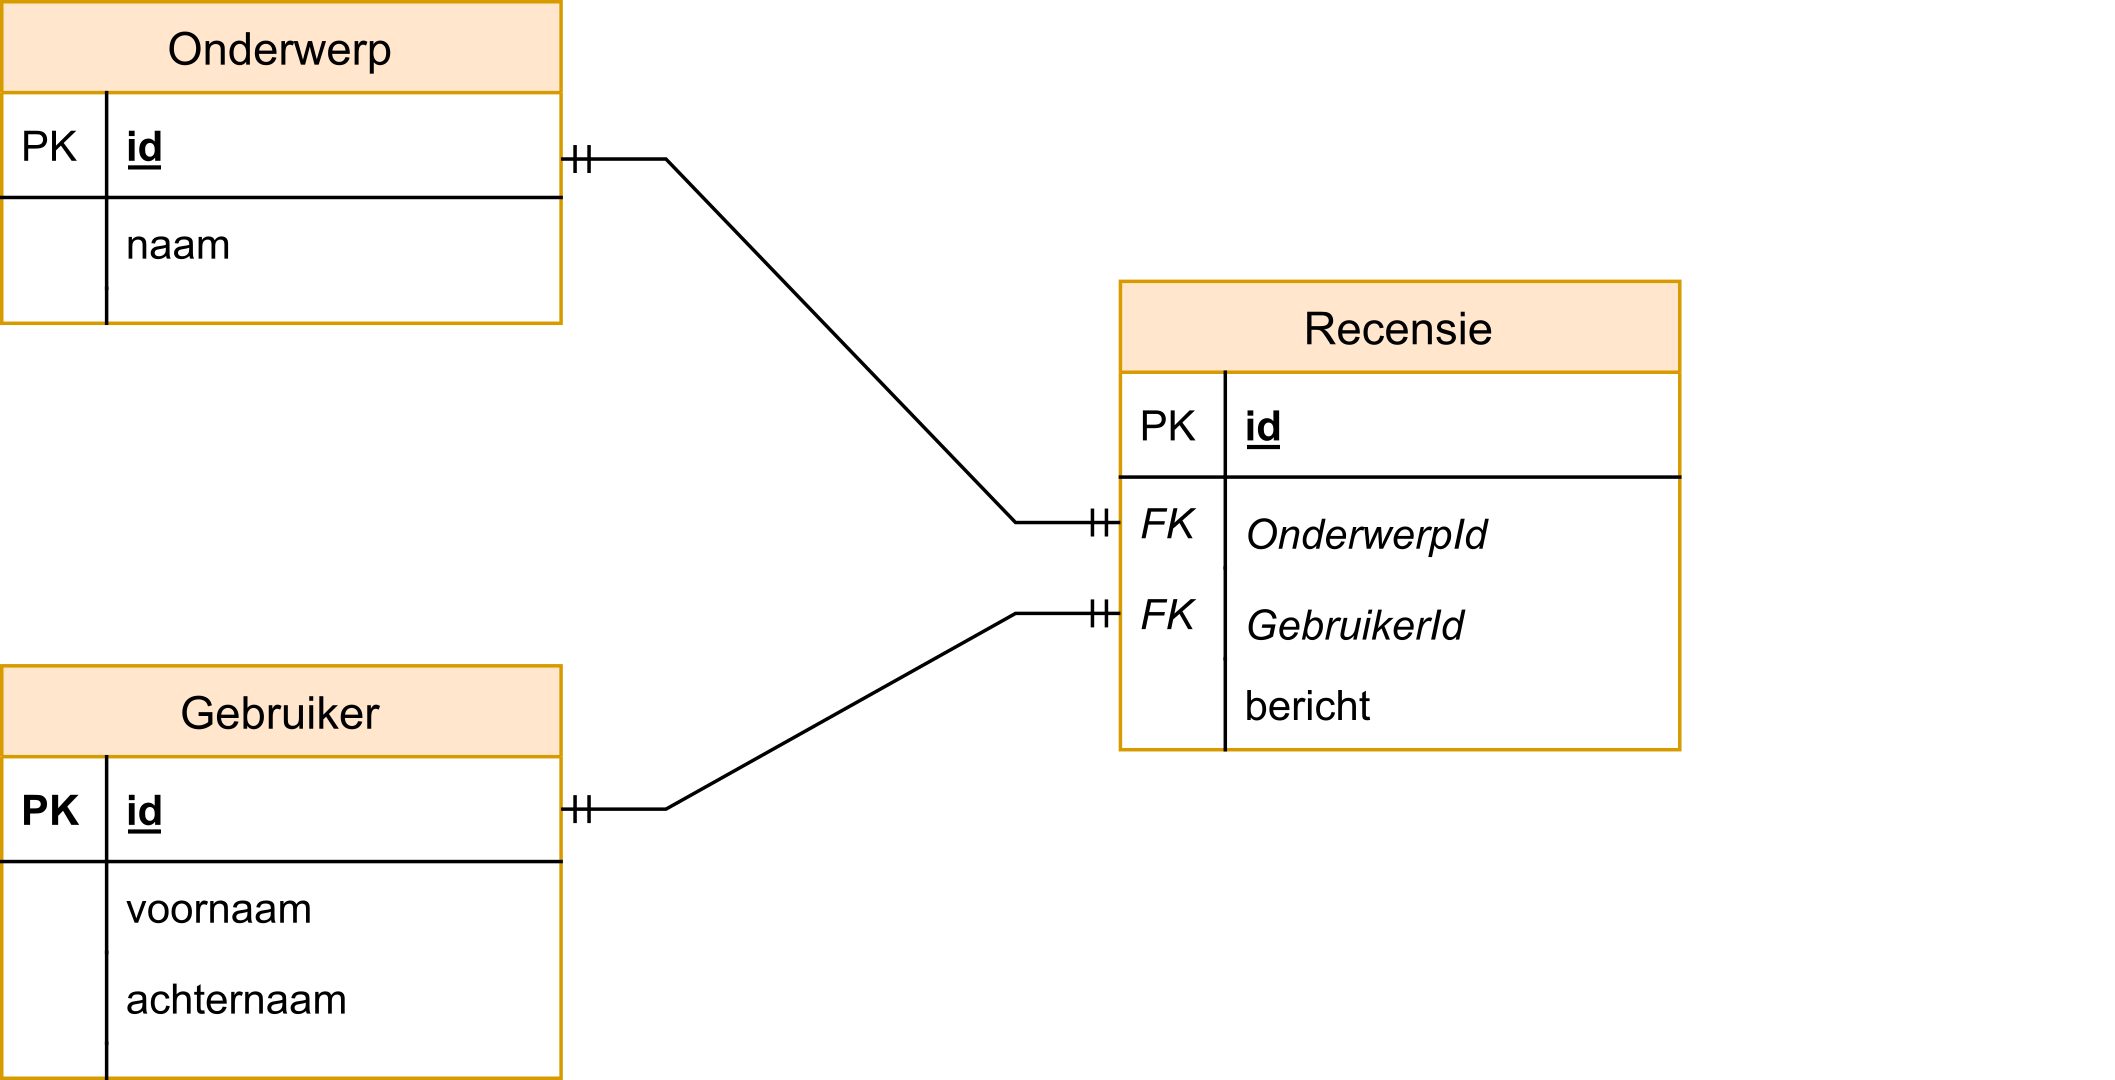
\includegraphics{graphics/erd.png}
  \caption{\label{fig:erd}ERD diagram van de recensie applicatie}
\end{figure}
\begin{listing}[H]
  \centering
  \begin{minted}[bgcolor=bg,
      fontfamily=tt,
      linenos=true,
      numberblanklines=true,
      numbersep=5pt,
      gobble=0,
      framesep=2mm,
      tabsize=4,
      obeytabs=false,
      breaklines=true,
      mathescape=false
      samepage=false,
      showspaces=false,
      showtabs =false,
      texcl=false]{js}
const { Model, DataTypes  } = require("sequelize");

class Gebruiker extends Model {}

async function GebruikerInit(sequelize) {
  Gebruiker.init(
    {
      id: {
        type: DataTypes.INTEGER,
        autoIncrement: true,
        primaryKey: true,
      },
      voornaam: {
        type: DataTypes.STRING,
        allowNull: false,
      },
      achternaam: {
        type: DataTypes.STRING,
      },
    },
    { sequelize, modelName: "Gebruiker" }
  );
  await Gebruiker.sync();
}

module.exports = {
  Gebruiker,
  GebruikerInit,
};
\end{minted}
\caption{\label{code:User}Code van het gebruiker model}
\end{listing}

\begin{listing}[H]
  \centering
  \begin{minted}[bgcolor=bg,
      fontfamily=tt,
      linenos=true,
      numberblanklines=true,
      numbersep=5pt,
      gobble=0,
      framesep=2mm,
      tabsize=4,
      obeytabs=false,
      breaklines=true,
      mathescape=false
      samepage=false,
      showspaces=false,
      showtabs =false,
      texcl=false]{js}
const { Model, DataTypes } = require("sequelize");

class Onderwerp extends Model {}

async function OnderwerpInit(sequelize) {
  Onderwerp.init(
    {
      id: {
        type: DataTypes.INTEGER,
        autoIncrement: true,
        primaryKey: true,
      },
      naam: {
        type: DataTypes.STRING,
        allowNull: false,
      },
    },
    { sequelize, modelName: "Onderwerp" }
  );
  await Onderwerp.sync();
}

module.exports = {
  Onderwerp,
  OnderwerpInit,
};
\end{minted}
\caption{\label{code:Subject}Code van het onderwerp model}
\end{listing}

\begin{listing}[H]
  \centering
  \begin{minted}[bgcolor=bg,
      fontfamily=tt,
      linenos=true,
      numberblanklines=true,
      numbersep=5pt,
      gobble=0,
      framesep=2mm,
      tabsize=4,
      obeytabs=false,
      breaklines=true,
      mathescape=false
      samepage=false,
      showspaces=false,
      showtabs =false,
      texcl=false]{js}
const { Model, DataTypes } = require("sequelize");
const { Gebruiker } = require("./gebruiker.js");
const { Onderwerp } = require("./onderwerp.js");
class Recensie extends Model {}

module.exports = async (sequelize) => {
  Recensie.init(
    {
      id: {
        type: DataTypes.INTEGER,
        autoIncrement: true,
        primaryKey: true,
      },
      bericht: {
        type: DataTypes.STRING,
        allowNull: false,
      },
    },
    { sequelize, modelName: "Recensie" }
  );
  Recensie.belongsTo(Gebruiker, { onDelete: "CASCADE" });
  Recensie.belongsTo(Onderwerp, { onDelete: "CASCADE" });
  await Recensie.sync();
};
\end{minted}
\caption{\label{code:Review}Code van het recensie model}
\end{listing}

In de code ~\ref{code:Instantie} wordt een connectie aangemaakt met de databank door het gebruik van Sequelize. 
De benodigde configuratie wordt met behulp van de config package opgehaald. Zo is de 
gebruikersnaam, databasenaam en de technologie van de database te vinden in de configuratie bestanden.
Voor zowel te kunnen werken met MySQL als Postgres wordt gebruikgemaakt van de packages: mysql2 en pg.
Het wachtwoord zal dankzij de config package opgehaald worden uit het environment om zo de veiligheid te waarborgen.
Deze configuratie wordt dan gebruikt om de connectie aan te maken en de tabellen te initializeren.
Nadien worden ook de gebruiker en onderwerp tabel opgevuld met voorbeeld data zoals te zien is in ~\ref{code:Seed}.

\begin{listing}[H]
  \centering
  \begin{minted}[bgcolor=bg,
      fontfamily=tt,
      linenos=true,
      numberblanklines=true,
      numbersep=5pt,
      gobble=0,
      framesep=2mm,
      tabsize=4,
      obeytabs=false,
      breaklines=true,
      mathescape=false
      samepage=false,
      showspaces=false,
      showtabs =false,
      texcl=false]{js}
const { Sequelize } = require("sequelize");
const configuration = require("config");
const RecensieMigratie = require("./recensie");
const seed = require("./seeder");
const { GebruikerInit } = require("./gebruiker");
const { OnderwerpInit } = require("./onderwerp");
//config
const username = configuration.get("username");
const database = configuration.get("database");
const dialect = configuration.get("dialect");
const password = configuration.get("password");

// Instantie aanmaken
let sequelize;
async function initializeSequelize() {
  sequelize = new Sequelize(database, username, password, {
    host: dialect,
    dialect: dialect,
    pool: {
      max: 100,
    }
  });
  try {
    await sequelize.authenticate();
    console.log("Connection has been established successfully.");
  } catch (error) {
    console.error("Unable to connect to the database:", error);
  }
  await GebruikerInit(sequelize);
  await OnderwerpInit(sequelize);
  await RecensieMigratie(sequelize);
  await seed(sequelize);
  return sequelize;
}

function getSequelize() {
  if (!sequelize) {
    throw new Error("initialize sequelize");
  }
  return sequelize;
}
module.exports = {
  initializeSequelize,
  getSequelize,
};
\end{minted}
\caption{\label{code:Instantie}Code bij aanmaken instantie sequelize}
\end{listing}

\begin{listing}[H]
  \centering
  \begin{minted}[bgcolor=bg,
      fontfamily=tt,
      linenos=true,
      numberblanklines=true,
      numbersep=5pt,
      gobble=0,
      framesep=2mm,
      tabsize=4,
      obeytabs=false,
      breaklines=true,
      mathescape=false
      samepage=false,
      showspaces=false,
      showtabs =false,
      texcl=false]{js}
async function seed(sequelize) {
  // Originele staat
  await sequelize.models.Gebruiker.destroy({ truncate: { cascade: true } });
  await sequelize.models.Onderwerp.destroy({ truncate: { cascade: true } });
  await sequelize.models.Gebruiker.create({
    id: 1,
    voornaam: "Quinten",
    achternaam: "De Wolf",
  });
  await sequelize.models.Onderwerp.create({
    id: 1,
    naam: "Cars",
  });
  await sequelize.models.Onderwerp.create({
    id: 2,
    naam: "Planes",
  });
  await sequelize.models.Onderwerp.create({
    id: 3,
    naam: "Racing",
  });
}
module.exports = seed;
\end{minted}
\caption{\label{code:Seed}Code bij het opvullen van de tabellen}
\end{listing}

Als laatste wordt de server aangemaakt om een POST methode op het recensie endpoint en een GET methode op het onderwerpen endpoint aan te nemen.
In ~\ref{code:NodeServer} wordt de code om dit te bereiken in Node.js getoond. Hierbij komt data in de vorm van JSON binnen voor de POST methode.
Deze bevat de recensie in combinatie met het id van het onderwerp en de gebruiker.
Deze zal dan gebruikt worden om een nieuwe rij aan te maken in de recensie tabel.
Daarnaast is er ook een GET endpoint die de lijst van alle onderwerpen zal ophalen en teruggeven.
In ~\ref{code:BunServer} kan dezelfde functionele code worden gevonden voor Bun.

\begin{listing}[H]
  \centering
  \begin{minted}[bgcolor=bg,
      fontfamily=tt,
      linenos=true,
      numberblanklines=true,
      numbersep=5pt,
      gobble=0,
      framesep=2mm,
      tabsize=4,
      obeytabs=false,
      breaklines=true,
      mathescape=false
      samepage=false,
      showspaces=false,
      showtabs =false,
      texcl=false]{js}
const http = require("node:http");
const { initializeSequelize } = require("./sequelize.js");
async function main() {
  const sequelizeInstance = await initializeSequelize();
  http
    .createServer(async (req, res) => {
      if (req.method === "POST" && req.url === "/recensie") {
        let body = "";
        req.on("data", (data) => {
          body += data.toString(); 
        });
        req.on("end", async () => {
          try {
            const data = JSON.parse(body);
            await sequelizeInstance.models.Recensie.create(data);
            res.writeHead(201, { "Content-Type": "application/json" });
            res.end();
          } catch (error) {
            console.error("Error:", error);
            res.writeHead(400, { "Content-Type": "application/json" });
            res.end(JSON.stringify({ message: "Invalid data" }));
          }
        });
      } else if (req.method === "GET" && req.url === "/onderwerpen") {
        try {
          const data = await sequelizeInstance.models.Onderwerp.findAll();
          res.writeHead(200, { "Content-Type": "application/json" });
          res.end(JSON.stringify(data));
        } catch {
          res.writeHead(500, { "Content-Type": "tet/plain" });
          res.end('Internal Server error')
        }
      }
    })
    .listen(3000);
}
main();
\end{minted}
\caption{\label{code:NodeServer}Code om de verzoeken te ontvangen binnen Node.js}
\end{listing}
\begin{listing}[H]
  \centering
  \begin{minted}[bgcolor=bg,
      fontfamily=tt,
      linenos=true,
      numberblanklines=true,
      numbersep=5pt,
      gobble=0,
      framesep=2mm,
      tabsize=4,
      obeytabs=false,
      breaklines=true,
      mathescape=false
      samepage=false,
      showspaces=false,
      showtabs =false,
      texcl=false]{js}
const { initializeSequelize } = require("./sequelize.js");
const sequelizeInstance = await initializeSequelize();
Bun.serve({
    port:3000,
    async fetch(request) {
        try {
            const url = new URL(request.url);
            if (request.method === "POST" && url.pathname === "/recensie") {
                const data = await request.json();
                await sequelizeInstance.models.Recensie.create(data);
                return new Response('',{headers: { "Content-Type": "application/json"}, status: 201});
            } else if (request.method === "GET" && url.pathname === "/onderwerpen") {
                const data = await sequelizeInstance.models.Onderwerp.findAll();
                return Response.json(data);
            }
        } catch (error) {
            console.error("Error:", error);
            return new Response(JSON.stringify({ message: 'Invalid data'}), 
            {headers: { "Content-Type": "application/json"}, status: 400})
        }
    }
})
\end{minted}
\caption{\label{code:BunServer}Code om de verzoeken te ontvangen binnen server}
\end{listing}
\subsection{Uitvoering metingen}
Voor de metingen wordt gebruikgemaakt van 2 hulpprogramma's: Hyperfine en Bombardier.
In \ref{code:HyperfineScript} wordt Hyperfine gebruikt om de gemiddelde uitvoeringstijd over verschillende iteraties van het script te berekenen.
Ook zal Hyperfine gebruikt worden om de gemiddelde installatietijd van de respectievelijke package managers te vergelijken zoals 
te zien is in \ref{code:HyperfineInstall}. Specifiek wordt de installatietijd bekeken wanneer het cache geheugen data bevat.
Bij de metingen wordt telkens versie 1.18 van Hyperfine gebruikt.
\begin{listing}[H]
  \centering
  \begin{minted}[bgcolor=bg,
      fontfamily=tt,
      linenos=true,
      numberblanklines=true,
      numbersep=5pt,  
      gobble=0,
      framesep=2mm,
      tabsize=4,
      obeytabs=false,
      breaklines=true,
      mathescape=false
      samepage=false,
      showspaces=false,
      showtabs =false,
      texcl=false]{shell-session}
> hyperfine --warmup 1 'node index.js 1000' 'bun index.js 1000'
      \end{minted}
      \caption{\label{code:HyperfineScript}Gebruik Hyperfine commando bij het script}
\end{listing}

\begin{listing}[H]
  \centering
  \begin{minted}[bgcolor=bg,
      fontfamily=tt,
      linenos=true,
      numberblanklines=true,
      numbersep=5pt,  
      gobble=0,
      framesep=2mm,
      tabsize=4,
      obeytabs=false,
      breaklines=true,
      mathescape=false
      samepage=false,
      showspaces=false,
      showtabs =false,
      texcl=false]{shell-session}
> hyperfine --prepare 'rm -rf node_modules' --warmup 1 --runs 100 'npm install' 'bun install'
      \end{minted}
      \caption{\label{code:HyperfineInstall}Gebruik Hyperfine commando bij het script}
\end{listing}
Daarnaast wordt voor de HTTP server gebruikgemaakt van Bombardier. 
Hierbij kan ingesteld worden hoeveel gelijktijdige connecties er zijn en hoeveel verzoeken per test worden verstuurd.
In de metingen zal getest worden door 500000 verzoeken te sturen met 10, 50 en 100 gelijktijdige connecties.
De commando's hiervoor zijn terug te vinden in \ref{code:Bombardier10}, \ref{code:Bombardier100} en \ref{code:Bombardier1000}.
Hierbij wordt telkens een POST verzoek gestuurd, in \ref{code:Bombardier10GET} wordt een voorbeeld getoond om GET verzoeken te sturen.
Bij de metingen wordt hiervoor gebruikgemaakt van versie 1.2.6 van Bombardier.
\begin{listing}[H]
  \centering
  \begin{minted}[bgcolor=bg,
      fontfamily=tt,
      linenos=true,
      numberblanklines=true,
      numbersep=5pt,  
      gobble=0,
      framesep=2mm,
      tabsize=4,
      obeytabs=false,
      breaklines=true,
      mathescape=false
      samepage=false,
      showspaces=false,
      showtabs =false,
      texcl=false]{shell-session}
> bombardier -c 10 -n 500000 -m POST -b '{"bericht": "test","GebruikerId": 1,"OnderwerpId": 1}' -l http://localhost:3000/recensie
      \end{minted}
      \caption{\label{code:Bombardier10}Gebruik Bombardier commando met 500000 verzoeken en 10 gelijktijdige connecties voor een POST verzoek}
\end{listing}
\begin{listing}[H]
  \centering
  \begin{minted}[bgcolor=bg,
      fontfamily=tt,
      linenos=true,
      numberblanklines=true,
      numbersep=5pt,  
      gobble=0,
      framesep=2mm,
      tabsize=4,
      obeytabs=false,
      breaklines=true,
      mathescape=false
      samepage=false,
      showspaces=false,
      showtabs =false,
      texcl=false]{shell-session}
> bombardier -c 50 -n 500000 -m POST -b '{"bericht": "test","GebruikerId": 1,"OnderwerpId": 1}' -l http://localhost:3000/recensie
      \end{minted}
      \caption{\label{code:Bombardier100}Gebruik Bombardier commando met 500000 verzoeken en 50 gelijktijdige connecties voor een POST verzoek}
\end{listing}
\begin{listing}[H]
  \centering
  \begin{minted}[bgcolor=bg,
      fontfamily=tt,
      linenos=true,
      numberblanklines=true,
      numbersep=5pt,  
      gobble=0,
      framesep=2mm,
      tabsize=4,
      obeytabs=false,
      breaklines=true,
      mathescape=false
      samepage=false,
      showspaces=false,
      showtabs =false,
      texcl=false]{shell-session}
> bombardier -c 100 -n 500000 -m POST -b '{"bericht": "test","GebruikerId": 1,"OnderwerpId": 1}' -l http://localhost:3000/recensie
      \end{minted}
      \caption{\label{code:Bombardier1000}Gebruik Bombardier commando met 500000 verzoeken en 100 gelijktijdige connecties voor een POST verzoek}
\end{listing}
\begin{listing}[H]
  \centering
  \begin{minted}[bgcolor=bg,
      fontfamily=tt,
      linenos=true,
      numberblanklines=true,
      numbersep=5pt,  
      gobble=0,
      framesep=2mm,
      tabsize=4,
      obeytabs=false,
      breaklines=true,
      mathescape=false
      samepage=false,
      showspaces=false,
      showtabs =false,
      texcl=false]{shell-session}
> bombardier -c 10 -n 500000 -l http://localhost:3000/onderwerpen
      \end{minted}
      \caption{\label{code:Bombardier10GET}Gebruik Bombardier commando met 500000 verzoeken en 10 gelijktijdige connecties voor een GET verzoek}
\end{listing}
Bij de uitvoering wordt gewerkt met een vorm van containervirtualisatie genaamd Docker.
Hierbij zit elke aplicatie in zijn eigen container waarbij aan de hand van een Dockerfile deze telkens wordt opgezet.
In \ref{code:dockerscript} is de Dockerfile voor het Quick Sort algoritme te zien. 
Hierbij wordt vertrokken van een omgeving die Node.js al bevat waar nadien Hyperfine en Bun worden geïnstalleerd.
Hierna wordt dan met behulp van Hyperfine de uitvoeringstijd van Bun en Node.js berekend.
Dit bestand moet eerst gebouwd worden met het docker build commando waarvan een voorbeeld te vinden is in \ref{code:dockerbuild}.
Daarna moet de image worden uitgevoerd met het docker run commando zoals het voorbeeld in \ref{code:dockerrun}.
Voor de HTTP server is er nog een bijkomend
Docker Compose bestand \ref{code:dockerscript} waar aan de hand van het commando in \ref{code:dockercompose}
zowel de databank als de server kan worden opgestart. Een voorbeeld hiervan voor zowel een MysSQL database als een PostgreSQL database is 
respectievelijk te zien in \ref{code:dockercomposefile} en \ref{code:dockercomposepostgres}.
Hiernaast wordt dan ook een Dockerfile gebruikt om de server te starten. De Dockerfile voor de Node.js en Bun server is te vinden in
respectievelijk \ref{code:dockernode} en \ref{code:dockerbun}. 
Om het gemiddelde CPU-gebruik en het maximale geheugengebruik te bepalen wordt het bombardier commando samen met het docker stats commando uitgevoerd in een zsh script.
Hierbij wordt voordat het bombardier commando wordt uitgevoerd de monitoring gestart van het geheugen en het cpu-gebruik. Nadien wordt het gemiddelde cpu-gebruik en het maximale geheugen gebruik bepaald.
Een voorbeeld van dit script  is te vinden in \ref{code:zshscript}. 
In dit voorbeeld wordt zowel de bombardier om de POST methode als de GET methode weergegeven. Afhankelijk van wat gemeten wordt, moet tussen 1 van deze 2 methoden gekozen worden.
Het aantal connecties kan als argument meegegeven worden bij de uitvoering van het script.
Daarnaast wordt bij de server ook de installatietijd van de package managers gemeten met de Dockerfile \ref{code:dockerinstall}.
Hiervoor wordt ook Hyperfine gebruikt waarbij de cache al wordt opgevuld door de warmup in het commando.
Tot slot wordt voor het maximaal geheugengebruik bij het script het zsh time commando gebruikt. Hierbij wordt de omgevingsvariabele 
ingesteld zodat het maximaal geheugengebruik kan getoond worden zoals in \ref{code:zshmemory}
\begin{listing}[H]
  \centering
  \begin{minted}[bgcolor=bg,
      fontfamily=tt,
      linenos=true,
      numberblanklines=true,
      numbersep=5pt,  
      gobble=0,
      framesep=2mm,
      tabsize=4,
      obeytabs=false,
      breaklines=true,
      mathescape=false
      samepage=false,
      showspaces=false,
      showtabs =false,
      texcl=false]{bash}
# Base image met Node.js geïnstalleerd
FROM node:21

# Installeer Hyperfine met apt
RUN apt-get update && \
    apt-get install -y curl && \
    apt-get install -y hyperfine
# Zet de werk map in de container
WORKDIR /app

# Download bun
RUN curl -fsSL https://bun.sh/install | bash && \
  ln -s $HOME/.bun/bin/bun /usr/local/bin/bun

# Kopieer de applicatie code naar de container
COPY . .
RUN ~/.bun/bin/bun install
# Commando dat wordt uitgevoerd wanneer container start
CMD ["hyperfine","--warmup", "1", "node index.js 1000", "bun index.js 1000"]
      \end{minted}
      \caption{\label{code:dockerscript}Dockerfile voor het Quick Sort algoritme}
\end{listing}
\begin{listing}[H]
  \centering
  \begin{minted}[bgcolor=bg,
      fontfamily=tt,
      linenos=true,
      numberblanklines=true,
      numbersep=5pt,  
      gobble=0,
      framesep=2mm,
      tabsize=4,
      obeytabs=false,
      breaklines=true,
      mathescape=false
      samepage=false,
      showspaces=false,
      showtabs =false,
      texcl=false]{shell-session}
> docker build -f "Dockerfile" -t testimage .
      \end{minted}
      \caption{\label{code:dockerbuild}Voorbeeld bouwen van een docker image met naam testimage}
\end{listing}
\begin{listing}[H]
  \centering
  \begin{minted}[bgcolor=bg,
      fontfamily=tt,
      linenos=true,
      numberblanklines=true,
      numbersep=5pt,  
      gobble=0,
      framesep=2mm,
      tabsize=4,
      obeytabs=false,
      breaklines=true,
      mathescape=false
      samepage=false,
      showspaces=false,
      showtabs =false,
      texcl=false]{shell-session}
> docker run -it testimage .
      \end{minted}
      \caption{\label{code:dockerrun}Voorbeeld uitvoeren van een docker image met naam testimage}
\end{listing}

\begin{listing}[H]
  \centering
  \begin{minted}[bgcolor=bg,
      fontfamily=tt,
      linenos=true,
      numberblanklines=true,
      numbersep=5pt,  
      gobble=0,
      framesep=2mm,
      tabsize=4,
      obeytabs=false,
      breaklines=true,
      mathescape=false
      samepage=false,
      showspaces=false,
      showtabs =false,
      texcl=false]{shell-session}
> docker-compose -f docker-compose.yml up --build
      \end{minted}
      \caption{\label{code:dockercompose}Uitvoeren van een docker compose}
\end{listing}
\begin{listing}[H]
  \centering
  \begin{minted}[bgcolor=bg,
      fontfamily=tt,
      linenos=true,
      numberblanklines=true,
      numbersep=5pt,  
      gobble=0,
      framesep=2mm,
      tabsize=4,
      obeytabs=false,
      breaklines=true,
      mathescape=false
      samepage=false,
      showspaces=false,
      showtabs =false,
      texcl=false]{yaml}
version: '3'

services:
  mysql:
    image: mysql:latest
    environment:
      MYSQL_ROOT_PASSWORD: Test12345
      MYSQL_DATABASE: review
    ports:
      - "3306:3306"
    healthcheck:
      test: ["CMD", "mysqladmin", "ping", "-h", "localhost"]
      interval: 5s
      timeout: 3s
      retries: 5

  bun:
    build: .
    depends_on:
      mysql:
        condition: service_healthy
    ports:
      - "3000:3000"
    environment:
      DB_PORT: 3306
      DB_USER: root
      DB_PASSWORD: Test12345
      DB_DATABASE: review
      DB_DIALECT: mysql
      \end{minted}
      \caption{\label{code:dockercomposefile}Docker Compose bestand voor het opstarten van de MySQL database en server}
\end{listing}
\begin{listing}[H]
  \centering
  \begin{minted}[bgcolor=bg,
      fontfamily=tt,
      linenos=true,
      numberblanklines=true,
      numbersep=5pt,  
      gobble=0,
      framesep=2mm,
      tabsize=4,
      obeytabs=false,
      breaklines=true,
      mathescape=false
      samepage=false,
      showspaces=false,
      showtabs =false,
      texcl=false]{yaml}
version: '3'

services:
  postgres:
    image: postgres:latest
    environment:
      POSTGRES_PASSWORD: Test12345
      POSTGRES_DB: review
      PGDATA: /data/postgres
    ports:
      - "5432:5432"
    healthcheck:
      test: ["CMD-SHELL", "pg_isready -U postgres"]
      interval: 5s
      timeout: 3s
      retries: 5

  bun:
    build: .
    depends_on:
      postgres:
        condition: service_healthy
    ports:
      - "3000:3000"
    environment:
      DB_PORT: 5432
      DB_USER: postgres
      DB_PASSWORD: Test12345
      DB_DATABASE: review
      DB_DIALECT: postgres
      \end{minted}
      \caption{\label{code:dockercomposepostgres}Docker Compose bestand voor het opstarten van de PostgreSQL database en server}
\end{listing}
\begin{listing}[H]
  \centering
  \begin{minted}[bgcolor=bg,
      fontfamily=tt,
      linenos=true,
      numberblanklines=true,
      numbersep=5pt,  
      gobble=0,
      framesep=2mm,
      tabsize=4,
      obeytabs=false,
      breaklines=true,
      mathescape=false
      samepage=false,
      showspaces=false,
      showtabs =false,
      texcl=false]{bash}
# Base image met Node.js geïnstalleerd
FROM node:21

# Zet de werk map in de container
WORKDIR /app

# Kopieer de package.json and package-lock.json bestanden naar de container
COPY package*.json ./

# Installeer dependencies
RUN npm install

# Kopieer de rest van de applicatie code naar de container
COPY . .

# Zet de poort open
EXPOSE 3000

# Commando dat wordt uitgevoerd wanneer container start
CMD ["npm", "run", "dev"]
      \end{minted}
      \caption{\label{code:dockernode}Dockerfile voor de node server}
\end{listing}


\begin{listing}[H]
  \centering
  \begin{minted}[bgcolor=bg,
      fontfamily=tt,
      linenos=true,
      numberblanklines=true,
      numbersep=5pt,  
      gobble=0,
      framesep=2mm,
      tabsize=4,
      obeytabs=false,
      breaklines=true,
      mathescape=false
      samepage=false,
      showspaces=false,
      showtabs =false,
      texcl=false]{bash}
# Base image met bun geïnstalleerd
FROM oven/bun:1.1.3 as base

# Zet de werk map in de container
WORKDIR /usr/src/app

# Kopieer de package.json and package-lock.json bestanden naar de container
COPY package.json bun.lockb ./
# Installeer dependencies
RUN bun install

# Kopieer de rest van de applicatie code naar de container
COPY . .

# Zet de poort open
EXPOSE 3000

# Commando dat wordt uitgevoerd wanneer container start
CMD ["bun", "run", "index.js"]
      \end{minted}
      \caption{\label{code:dockerbun}Dockerfile voor de bun server}
\end{listing}

\begin{listing}[H]
  \centering
  \begin{minted}[bgcolor=bg,
      fontfamily=tt,
      linenos=true,
      numberblanklines=true,
      numbersep=5pt,  
      gobble=0,
      framesep=2mm,
      tabsize=4,
      obeytabs=false,
      breaklines=true,
      mathescape=false
      samepage=false,
      showspaces=false,
      showtabs =false,
      texcl=false]{bash}
#!/bin/zsh

# Start de monitoring
docker stats <container_naam> --format "table {{.Container}}\t{{.CPUPerc}}\t{{.MemUsage}}" > container_stats.txt &

# Start bombardier POST
bombardier -c "$1" -n 500000 -m POST -b '{"bericht": "test","GebruikerId": 1,"OnderwerpId": 1}' -l http://localhost:3000/recensie
# Of
# Start bombardier GET
bombardier -c "$1" -n 500000 -l http://localhost:3000/onderwerpen

# Stop de docker stats

target_command="/Applications/Docker.app/Contents/Resources
/bin/com.docker.cli stats"
docker_cli_pid=$(ps aux | grep "$target_command" | grep -v grep | awk '{print $2}')

if [[ -n $docker_cli_pid ]]; then
    echo "Killing Docker CLI process with PID: $docker_cli_pid"
    kill -9 $docker_cli_pid
else
    echo "Docker CLI process not found."
fi


# Bereken gemiddeld CPU-gebruik en hoogste memory
while IFS= read -r line; do
    if [[ $line =~ ([0-9]+\.[0-9]+)%(.*[0-9]+\.[0-9]+)MiB ]]; then
        cpu_percent="${match[1]}"
        mem_usage="${match[2]}"
        cpu_percent_sum=$((cpu_percent_sum + cpu_percent))
        if (( mem_usage > highest_mem_usage )); then
            highest_mem_usage="$mem_usage"
        fi
        ((total_lines++))
    fi
done < container_stats.txt

average_cpu_percent=$((cpu_percent_sum / total_lines))

# Toon resultaten
echo "Gemiddelde CPU-gebruik: $average_cpu_percent%"
echo "Maximaal geheugen gebruik: $highest_mem_usage"

      \end{minted}
      \caption{\label{code:zshscript}Dockerfile voor het Quick Sort algoritme}
\end{listing}

\begin{listing}[H]
  \centering
  \begin{minted}[bgcolor=bg,
      fontfamily=tt,
      linenos=true,
      numberblanklines=true,
      numbersep=5pt,  
      gobble=0,
      framesep=2mm,
      tabsize=4,
      obeytabs=false,
      breaklines=true,
      mathescape=false
      samepage=false,
      showspaces=false,
      showtabs =false,
      texcl=false]{bash}
# Base image met Node.js geïnstalleerd
FROM node:21

# Installeer Hyperfine met apt
RUN apt-get update && \
    apt-get install -y curl && \
    apt-get install -y hyperfine
# Zet de werk map in de container
WORKDIR /app

RUN curl -fsSL https://bun.sh/install | bash && \
  ln -s $HOME/.bun/bin/bun /usr/local/bin/bun

# Kopieer de applicatiebestanden naar de container
COPY . .
RUN ~/.bun/bin/bun install
# Commando dat wordt uitgevoerd wanneer container start
CMD ["hyperfine","--prepare", "rm -rf node_modules", "--warmup","1","--runs","100","bun install","npm install"]
      \end{minted}
      \caption{\label{code:dockerinstall}Dockerfile voor de installatietijd te meten bij de server}
\end{listing}

\begin{listing}[H]
  \centering
  \begin{minted}[bgcolor=bg,
      fontfamily=tt,
      linenos=true,
      numberblanklines=true,
      numbersep=5pt,  
      gobble=0,
      framesep=2mm,
      tabsize=4,
      obeytabs=false,
      breaklines=true,
      mathescape=false
      samepage=false,
      showspaces=false,
      showtabs =false,
      texcl=false]{shell-session}
> TIMEFMT='%J   %U  user %S system %P cpu %*E total'$'\n'\
'max memory:                %M '$MAX_MEMORY_UNITS''$'\n'\
> time node index.js 1000
> time bun index.js 1000
      \end{minted}
      \caption{\label{code:zshmemory}Aanpassing zsh commando voor maximaal geheugengebruik te tonen}
\end{listing}

\subsection{Resultaten proof-of-concept}
In deze sectie zullen de resultaten van de performantie testen besproken worden.
Hierbij worden eerst de resultaten voor de uitvoeringstijd bij het Quick Sort algoritme bekeken.
Daarna worden de resultaten van de server besproken op vlak van uitvoeringstijd, cpu-gebruik, geheugengebruik, latentie en de installatietijd 
bij zowel het gebruik van een MySQL database als een PostgreSQL database.

\subsubsection{Resultaten  Quick Sort algoritme}
De resultaten voor de gemiddelde uitvoeringstijd bij het Quick Sort algoritme werden bekomen met behulp van Hyperfine.
Hierbij werd gekeken naar de uitvoeringstijd voor het sorteren van een array bestaande uit 1000 elementen met volgend commando \ref{code:HyperfineScript}..
Bun heeft hierbij een gemiddelde uitvoeringstijd van 6.4 milliseconden met een standaardafwijking van 0.8 milliseconden. 
Dit tegenover de gemiddelde uitvoeringstijd van 14.1 milleseconden bij Node.js met een standaardafwijking van 1.3 milliseconden.
In figuur \ref{fig:uitvoeringstijdscript} wordt de gemiddelde uitvoeringstijd per omgeving visueel voorgesteld
Daarbij is op te merken dat de gemiddelde uitvoeringstijd van Bun 2.21 keer sneller is dan bij Node.js.
In figuur \ref{fig:RAMscript} wordt het maximale geheugengebruik voor zowel Bun als Node.js weergegeven. 
Hierbij werd het time commando telkens 5 keer uitgevoerd.
Als resultaat heeft Bun met 30.69 MB een lager geheugengebruik dan Node.js met 36.4 MB.
\begin{figure}[H]
  \centering
  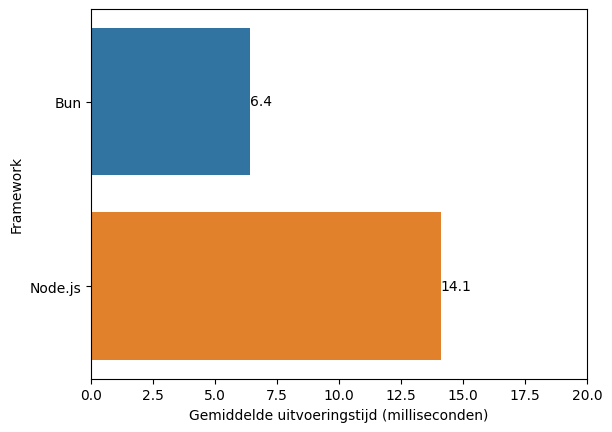
\includegraphics{graphics/scriptuitvoeringstijd.png}
  \caption{\label{fig:uitvoeringstijdscript}Gemiddelde uitvoeringstijd van het Quick Sort algoritme voor Bun en Node.js}
\end{figure}

\begin{figure}[H]
  \centering
  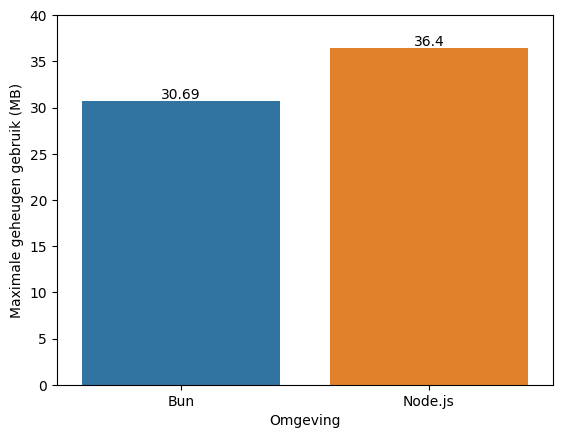
\includegraphics{graphics/RAMScript.png}
  \caption{\label{fig:RAMscript}Maximale geheugengebruik van het Quick Sort algoritme voor Bun en Node.js}
\end{figure}

\subsection{Resultaten Recensie applicatie}
De resultaten voor de gemiddelde installatietijd bij de p
ackage managers werden bekomen met behulp van Hyperfine.
Hierbij werd eerst een warmup uitvoering gedaan om de cache al op te vullen.
In figuur \ref{fig:installatietijdapp} zijn de resultaten visueel voorgesteld per omgeving.
Hierbij is op te merken dat Bun met een gemiddelde installatietijd van 24,9 milliseconden en een standaardafwijking van 2,4 milliseconden 24,5 keer sneller 
is dan Node.js met een gemiddelde installatietijd van 610,1 milleseconden en een standaardafwijking van 100,1 milliseconden.
\begin{figure}[H]
  \centering
  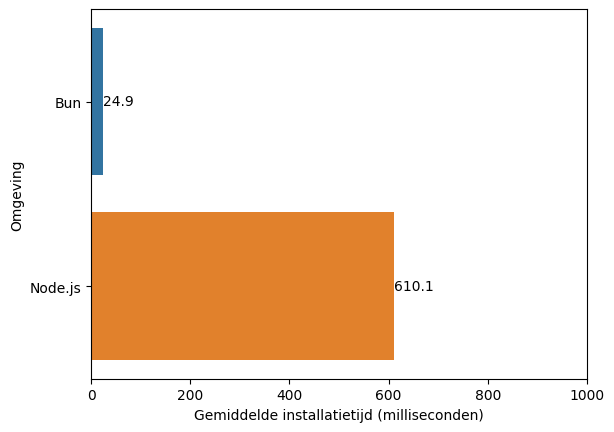
\includegraphics{graphics/install.png}
  \caption{\label{fig:installatietijdapp}Gemiddelde installatietijd van de packages in Bun en Node.js}
\end{figure}

Voor de andere resultaten werd gebruikgemaakt van Bombardier waarbij telkens met 10, 50 en 100 connecties 
500000 verzoeken werden gestuurd naar de server.

\subsubsection{Resultaten voor de applicatie met een MySQL database}
In deze sectie worden de bekomen resultaten van de applicatie besproken waarbij een MySQL database werd gebruikt.
In tabel \ref{tab:getbombardier} kunnen de resultaten gezien worden van de metingen waarbij de onderwerpen werden opgehaald aan de hand van een GET verzoek.
Er wordt gestreefd naar een zo hoog mogelijk aantal verzoeken per seconde met een zo laag mogelijke latentie, geheugengebruik en cpu-gebruik.
Zoals te zien scoort Bun op het vlak van aantal verzoeken per seconde en latentie beter dan Node.js ongeacht van het aantal connecties. 
Echter heeft Bun bij het aantal verzoeken per seconde wel telkens een grotere standaardafwijking en zijn er dus meer uitschieters aanwezig zijn.
Langs de andere kant verbruikt Bun telkens meer resources. Zo heeft Bun bij elke aantal connecties een hoger CPU-gebruik en zijn de pieken van het geheugen consistent hoger dan bij Node.js.
In figuren \ref{fig:getaantalverzoekenmysql}, \ref{fig:getaantallatentienmysql}, \ref{fig:getgeheugenmysql} en \ref{fig:getcpumysql} kunnen de visuele voorstellingen 
voor respectievelijk het aantal verzoeken per seconde, het aantal latentie, het maximale geheugengebruik en het gemiddeld CPU-gebruik worden gevonden.
\begin{table}[]
  \begin{tabular}{|c|cccccc|}
  \hline
  \multicolumn{1}{|l|}{}                                                                     & \multicolumn{1}{l}{} & Bun      & \multicolumn{1}{l|}{}    & \multicolumn{1}{l}{} & \multicolumn{1}{l}{Node.js} & \multicolumn{1}{l|}{} \\ \hline
  Aantal connecties                                                                          & 10                   & 50       & \multicolumn{1}{c|}{100} & 10                   & 50                          & 100                   \\ \hline
  \begin{tabular}[c]{@{}c@{}}Gemiddeld aantal \\ verzoeken per seconde\end{tabular}          & 9069.30              & 10489.67 & 9298.56                  & 7314.91              & 8985.16                     & 8500.49               \\ \cline{1-1}
  \begin{tabular}[c]{@{}c@{}}Standaardafwijking aantal \\ verzoeken per seconde\end{tabular} & 2974.14              & 3398.39  & 3063.49                  & 2930.06              & 2813.57                     & 2759.61               \\ \cline{1-1}
  \begin{tabular}[c]{@{}c@{}}Latentie \\ (milliseconden)\end{tabular}                        & 1.10                 & 4.76     & 10.76                    & 1.31                 & 5.56                        & 11.77                 \\ \cline{1-1}
  \begin{tabular}[c]{@{}c@{}}Standaardafwijking\\ latentie\\ (milliseconden)\end{tabular}    & 0.72090              & 1.94     & 3.17                     & 1.15                 & 1.63                        & 2.78                  \\ \cline{1-1}
  \begin{tabular}[c]{@{}c@{}}Maximale \\ geheugengebruik \\ (MB)\end{tabular}                & 110.7                & 175.7    & 261.7                    & 104.4                & 114.8                       & 133.3                 \\ \cline{1-1}
  \begin{tabular}[c]{@{}c@{}}Gemiddeld\\ CPU-gebruik\\ (\%)\end{tabular}                     & 110.4                & 112.25   & 116.09                   & 95.24                & 101.64                      & 102.7                 \\ \hline
  \end{tabular}
  \caption{\label{tab:getbombardier}Resultaten metingen waarbij onderwerpen worden opgehaald met een GET request uit de MySQL database.}
  \end{table}

  \begin{figure}[H]
    \centering
    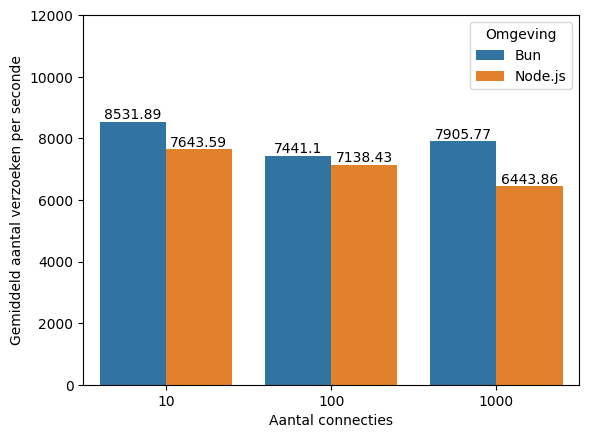
\includegraphics[width=0.7\columnwidth]{graphics/GetMySqlVerzoeken.png}
    \caption{\label{fig:getaantalverzoekenmysql}Visuele voorstelling gemiddeld aantal verzoeken per seconde bij het ophalen van de onderwerpen.}
  \end{figure}
  \begin{figure}[H]
    \centering
    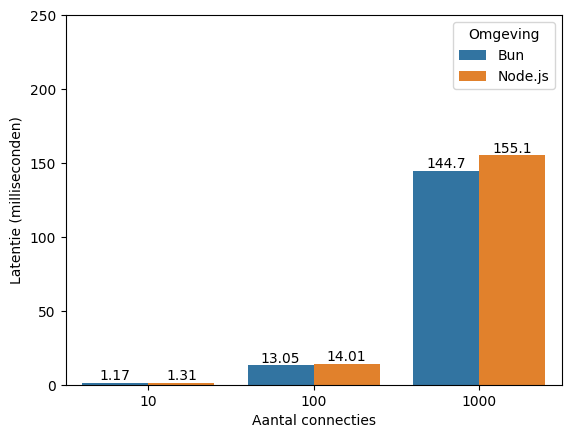
\includegraphics[width=0.7\columnwidth]{graphics/GetMySqlLatentie.png}
    \caption{\label{fig:getaantallatentienmysql}Visuele voorstelling gemiddelde latentie bij het ophalen van de onderwerpen.}
  \end{figure}
  \begin{figure}[H]
    \centering
    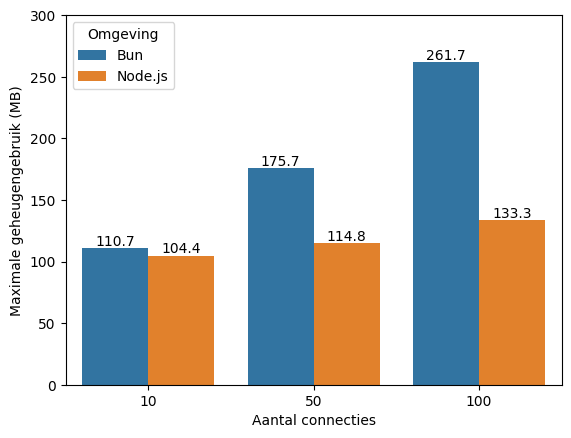
\includegraphics[width=0.7\columnwidth]{graphics/GetMySqlRAM.png}
    \caption{\label{fig:getgeheugenmysql}Visuele voorstelling maximale geheugen gebruik bij het ophalen van de onderwerpen.}
  \end{figure}
  \begin{figure}[H]
    \centering
    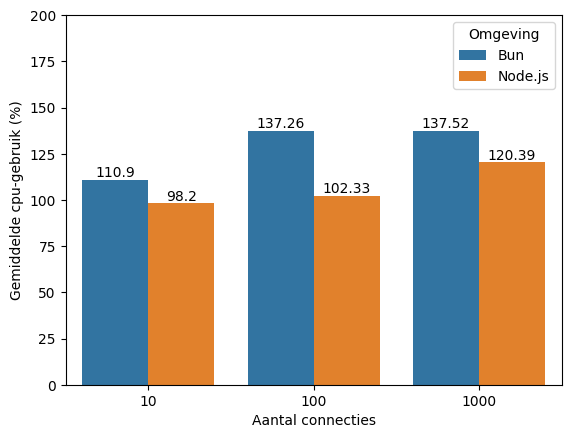
\includegraphics[width=0.7\columnwidth]{graphics/GetMySqlCpu.png}
    \caption{\label{fig:getcpumysql}Visuele voorstelling gemiddeld CPU-gebruik bij het ophalen van de onderwerpen.}
  \end{figure}

In tabel \ref{tab:postbombardier} kunnen de resultaten gezien worden van de metingen waarbij 
een gebruiker een recensie schrijft over een bepaald onderwerp door gebruik van een POST verzoek.
Hierbij is op te merken dat Bun op zowel het vlak van gemiddeld aantal verzoeken als latentie gelijkaardig scoort aan Node.js bij 10 connecties. Zo heeft Bun
een gemiddeld aantal verzoeken van 4483 terwijl Node.js hierbij een gemiddelde heeft van 4504.87 heeft. 
Ook bij de latentie is dit het geval waarbij Bun een latentie heeft van 2.27 milliseconden en Node.js een latentie van 2.22 milliseconden.
Deze trend zet zich echter niet voort bij de 50 en 100 connecties waarbij Bun steeds beter presteert op vlak van latentie en aantal verzoeken per seconde.
Echter zit er wel consistentie bij het geheugengebruik tussen het aantal connecties.
Bij 10 connecties heeft Bun al een geheugengebruik van 161.2MB terwijl Node.js hier maar een verbruik heeft van 138.2MB.
Voor de 50 en 100 connecties zit Bun telkens hoger dan Node.js.
Hetzelfde is te zien bij het gemiddeld CPU-gebruik voor de 50 en 100 connecties, waarbij Bun respectievelijk 109.43\% en 118.56\% heeft terwijl Node.js maar een gemiddelde van 98.4\% en 107.73\% CPU-gebruik heeft.
In figuren \ref{fig:postaantalverzoekenmysql}, \ref{fig:postaantallatentienmysql}, \ref{fig:postgeheugenmysql} en \ref{fig:postcpumysql} kunnen de visuele voorstellingen 
voor respectievelijk het aantal verzoeken per seconde, het aantal latentie, het maximale geheugengebruik en het gemiddeld CPU-gebruik worden gevonden.
\begin{table}[]
  \begin{tabular}{|c|cccccc|}
  \hline
  \multicolumn{1}{|l|}{}                                                                     & \multicolumn{1}{l}{} & Bun     & \multicolumn{1}{l|}{}    & \multicolumn{1}{l}{} & \multicolumn{1}{l}{Node.js} & \multicolumn{1}{l|}{} \\ \hline
  Aantal connecties                                                                          & 10                   & 50      & \multicolumn{1}{c|}{100} & 10                   & 50                          & 100                   \\ \hline
  \begin{tabular}[c]{@{}c@{}}Gemiddeld aantal \\ verzoeken per seconde\end{tabular}          & 4483                 & 5856.48 & 5902.12                  & 4504.87              & 5498.57                     & 5282.67               \\ \cline{1-1}
  \begin{tabular}[c]{@{}c@{}}Standaardafwijking aantal \\ verzoeken per seconde\end{tabular} & 904.95               & 2006.84 & 2204.15                  & 981.92               & 2032.85                     & 2226.43               \\ \cline{1-1}
  \begin{tabular}[c]{@{}c@{}}Latentie \\ (milliseconden)\end{tabular}                        & 2.27                 & 8.54    & 16.95                    & 2.22                 & 9.10                        & 18.94                 \\ \cline{1-1}
  \begin{tabular}[c]{@{}c@{}}Standaardafwijking\\ latentie\\ (milliseconden)\end{tabular}    & 1.17                 & 2.75    & 4.63                     & 1.10                 & 3.46                        & 16.81                 \\ \cline{1-1}
  \begin{tabular}[c]{@{}c@{}}Maximale \\ geheugengebruik \\ (MB)\end{tabular}                & 161.2                & 196.4   & 238.8                    & 138.2                & 115.85                      & 174.6                 \\ \cline{1-1}
  \begin{tabular}[c]{@{}c@{}}Gemiddeld\\ CPU-gebruik\\ (\%)\end{tabular}                     & 63.30                & 109.43  & 118.56                   & 66.26                & 98.4                        & 107.73                \\ \hline
  \end{tabular}
  \caption{\label{tab:postbombardier}Resultaten metingen waarbij door een bepaalde gebruiker een recensie over een onderwerp werd gemaakt in de MySQL database met een POST request.}
  \end{table}
    \begin{figure}[H]
      \centering
      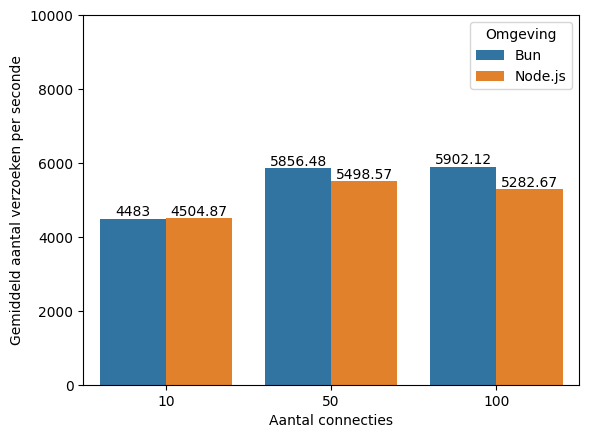
\includegraphics[width=0.7\columnwidth]{graphics/PostMySqlVerzoeken.png}
      \caption{\label{fig:postaantalverzoekenmysql}Visuele voorstelling gemiddeld aantal verzoeken per seconde bij het maken van een recensie.}
    \end{figure}
    \begin{figure}[H]
      \centering
      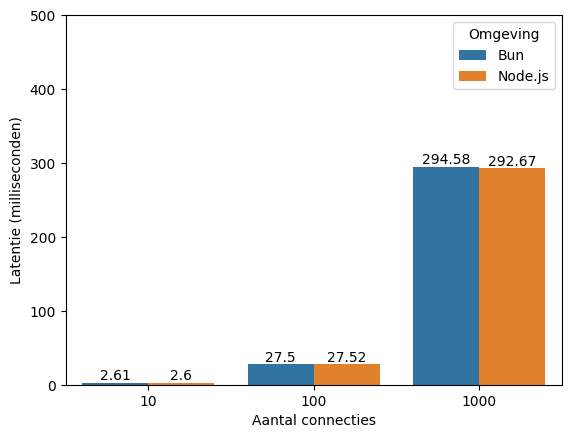
\includegraphics[width=0.7\columnwidth]{graphics/PostMySqlLatentie.png}
      \caption{\label{fig:postaantallatentienmysql}Visuele voorstelling gemiddelde latentie bij het maken van een recensie.}
    \end{figure}
    \begin{figure}[H]
      \centering
      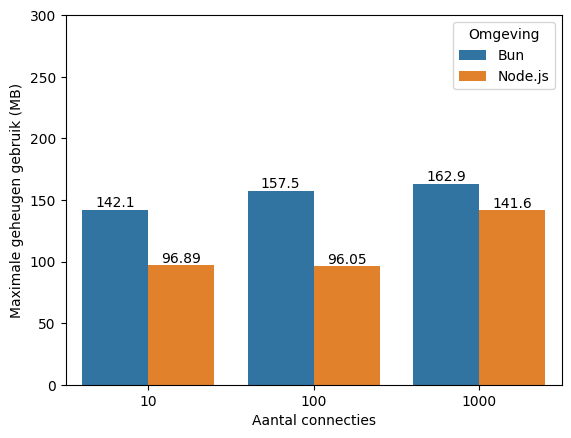
\includegraphics[width=0.7\columnwidth]{graphics/PostMySqlRAM.png}
      \caption{\label{fig:postgeheugenmysql}Visuele voorstelling maximale geheugen gebruik bij het maken van een recensie.}
    \end{figure}
    \begin{figure}[H]
      \centering
      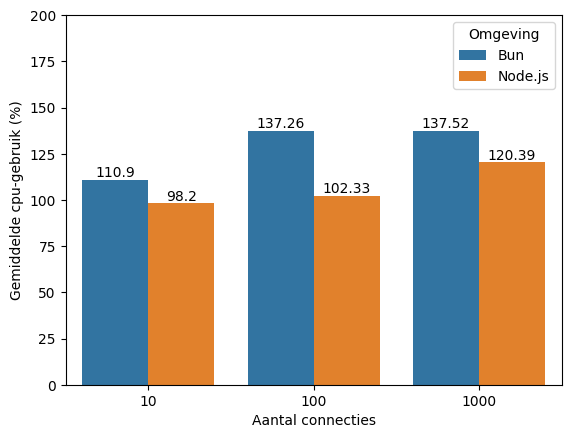
\includegraphics[width=0.7\columnwidth]{graphics/PostMySqlCpu.png}
      \caption{\label{fig:postcpumysql}Visuele voorstelling gemiddeld CPU-gebruik bij het maken van een recensie.}
    \end{figure}
\subsection{Resultaten voor de applicatie met een PostgreSQL database}
In deze sectie worden de bekomen resultaten van de applicatie besproken waarbij een PostgreSQL database werd gebruikt.
In tabel \ref{tab:getbombardierpostgres} kunnen de resultaten gezien worden van de metingen waarbij de onderwerpen werden opgehaald aan de hand van een GET verzoek.
Er wordt hierbij gestreefd naar een zo hoog mogelijk aantal verzoeken per seconde met een zo laag mogelijke latentie, geheugengebruik en cpu-gebruik.
Zoals te zien scoort Bun ook weer hier beter op zowel het vlak van aantal verzoeken per seconde als latentie.
Langs de andere kant verbruikt Bun telkens meer resources. Zo heeft Bun bij elke aantal connecties een hoger CPU-gebruik en zijn de pieken van het geheugen consistent hoger dan bij Node.js.
In figuren \ref{fig:getaantalverzoekenpostgres}, \ref{fig:getaantallatentienpostgres}, \ref{fig:getgeheugenpostgres} en \ref{fig:getcpupostgres} kunnen de visuele voorstellingen 
voor respectievelijk het aantal verzoeken per seconde, het aantal latentie, het maximale geheugengebruik en het gemiddeld CPU-gebruik worden gevonden.
\begin{table}[]
  \begin{tabular}{|c|cccccc|}
  \hline
  \multicolumn{1}{|l|}{}                                                                     & \multicolumn{1}{l}{} & Bun      & \multicolumn{1}{l|}{}    & \multicolumn{1}{l}{} & \multicolumn{1}{l}{Node.js} & \multicolumn{1}{l|}{} \\ \hline
  Aantal connecties                                                                          & 10                   & 50       & \multicolumn{1}{c|}{100} & 10                   & 50                          & 100                   \\ \hline
  \begin{tabular}[c]{@{}c@{}}Gemiddeld aantal \\ verzoeken per seconde\end{tabular}          & 9532.83              & 10681.12 & 10040                    & 8957.89              & 9925.63                     & 9605.79               \\ \cline{1-1}
  \begin{tabular}[c]{@{}c@{}}Standaardafwijking aantal \\ verzoeken per seconde\end{tabular} & 3047.08              & 3779.48  & 3626.49                  & 2529.11              & 3185.40                     & 3022.16               \\ \cline{1-1}
  \begin{tabular}[c]{@{}c@{}}Latentie \\ (milliseconden)\end{tabular}                        & 1.05                 & 4.68     & 9.96                     & 1.12                 & 5.04                        & 10.41                 \\ \cline{1-1}
  \begin{tabular}[c]{@{}c@{}}Standaardafwijking\\ latentie\\ (milliseconden)\end{tabular}    & 0.66886              & 1.94     & 3.02                     & 0.70591              & 1.98                        & 3.18                  \\ \cline{1-1}
  \begin{tabular}[c]{@{}c@{}}Maximale \\ geheugengebruik \\ (MB)\end{tabular}                & 160.5                & 189.9    & 203.3                    & 94.41                & 136.7                       & 149.9                 \\ \cline{1-1}
  \begin{tabular}[c]{@{}c@{}}Gemiddeld\\ CPU-gebruik\\ (\%)\end{tabular}                     & 111.87               & 117.71   & 122.40                   & 98.30                & 101.82                      & 104.81                \\ \hline
  \end{tabular}
  \caption{\label{tab:getbombardierpostgres}Resultaten metingen waarbij onderwerpen worden opgehaald met een GET request uit de PostgreSQL database.}
  \end{table}
  
  \begin{figure}[H]
    \centering
    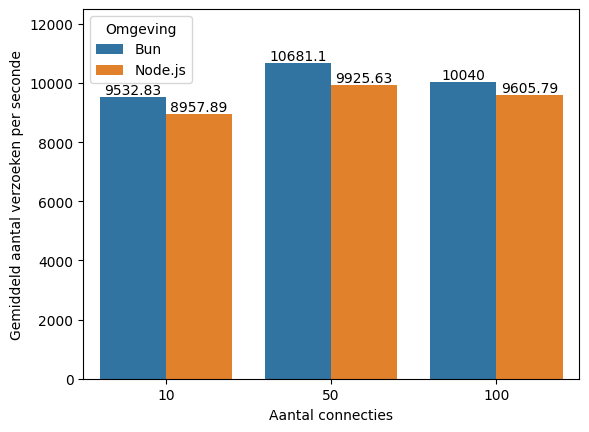
\includegraphics[width=0.7\columnwidth]{graphics/GetPostgresVerzoeken.png}
    \caption{\label{fig:getaantalverzoekenpostgres}Visuele voorstelling gemiddeld aantal verzoeken per seconde bij het ophalen van de onderwerpen.}
  \end{figure}
  \begin{figure}[H]
    \centering
    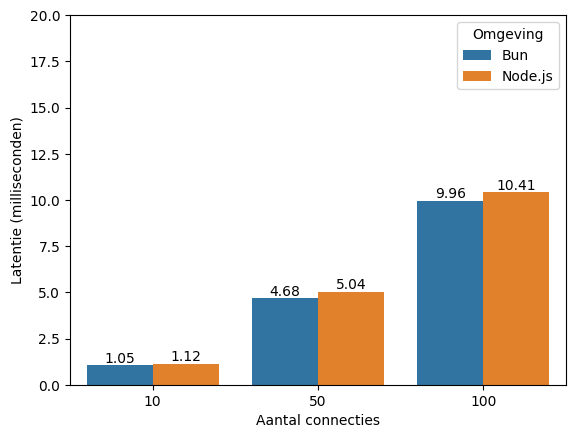
\includegraphics[width=0.7\columnwidth]{graphics/GetPostgresLatentie.png}
    \caption{\label{fig:getaantallatentienpostgres}Visuele voorstelling gemiddelde latentie bij het ophalen van de onderwerpen.}
  \end{figure}
  \begin{figure}[H]
    \centering
    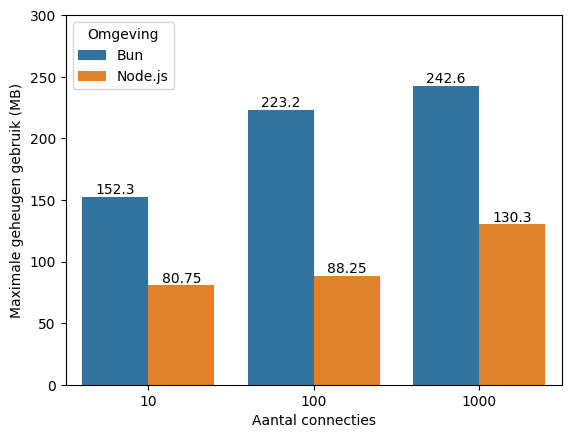
\includegraphics[width=0.7\columnwidth]{graphics/GetPostgresRAM.png}
    \caption{\label{fig:getgeheugenpostgres}Visuele voorstelling maximale geheugen gebruik bij het ophalen van de onderwerpen.}
  \end{figure}
  \begin{figure}[H]
    \centering
    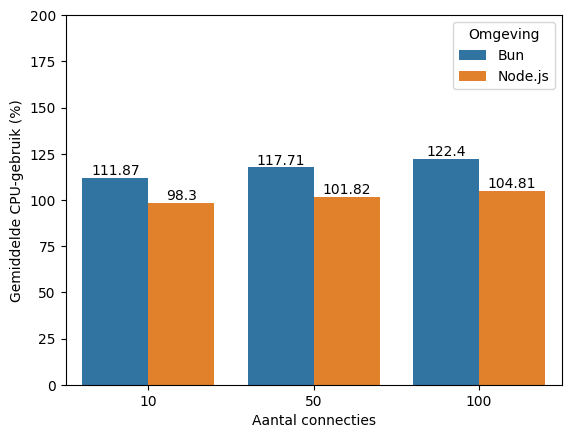
\includegraphics[width=0.7\columnwidth]{graphics/GetPostgresCpu.png}
    \caption{\label{fig:getcpupostgres}Visuele voorstelling gemiddeld CPU-gebruik bij het ophalen van de onderwerpen.}
  \end{figure}

In tabel \ref{tab:postbombardierpostgres} kunnen de resultaten gezien worden van de metingen waarbij 
een gebruiker een recensie schrijft over een bepaald onderwerp door gebruik van een POST verzoek en de PostgreSQL databank.
Hierbij scoort Bun bij alle aantallen connecties beter dan Node.js
Zo heeft Bun bij 10 connecties een gemiddelde van 5433.39 aantal verzoeken per seconde met een latentie van 1.84 milliseconden. 
Dit tegenover Node.js met een gemiddelde van 5221.94 verzoeken per seconde en een latentie van 1.91 milliseconden.
Deze trend zet zich voort bij zowel de 50 als 100 connecties.
Op vlak van middelengebruik is er ook hier een verschil. Echter scoort Node.js hierbij beter dan Bun.
 Zo heeft het bijvoorbeeld bij 100 connecties een maximaal geheugengebruik van 146.4MB en een gemiddeld CPU-gebruik van 104.75\%.
Bij Bun is dit hoger met een geheugengebruik van 179.2MB en een gemiddeld CPU-gebruik van 118.79\%.
In figuren \ref{fig:postaantalverzoekenpostgres}, \ref{fig:postaantallatentiepostgres}, \ref{fig:postgeheugenpostgres} en \ref{fig:postcpupostgres} kunnen de visuele voorstellingen 
voor respectievelijk het aantal verzoeken per seconde, het aantal latentie, het maximale geheugengebruik en het gemiddeld CPU-gebruik worden gevonden.
\begin{table}[]
  \begin{tabular}{|c|cccccc|}
  \hline
  \multicolumn{1}{|l|}{}                                                                     & \multicolumn{1}{l}{} & Bun     & \multicolumn{1}{l|}{}    & \multicolumn{1}{l}{} & \multicolumn{1}{l}{Node.js} & \multicolumn{1}{l|}{} \\ \hline
  Aantal connecties                                                                          & 10                   & 50      & \multicolumn{1}{c|}{100} & 10                   & 50                          & 100                   \\ \hline
  \begin{tabular}[c]{@{}c@{}}Gemiddeld aantal \\ verzoeken per seconde\end{tabular}          & 5433.39              & 6098.80 & 6170                     & 5221.94              & 5864.77                     & 5785.76               \\ \cline{1-1}
  \begin{tabular}[c]{@{}c@{}}Standaardafwijking aantal \\ verzoeken per seconde\end{tabular} & 1398.06              & 2151.57 & 2186.09                  & 1237.90              & 1866.52                     & 2023.42               \\ \cline{1-1}
  \begin{tabular}[c]{@{}c@{}}Latentie \\ (milliseconden)\end{tabular}                        & 1.84                 & 8.20    & 16.22                    & 1.91                 & 8.53                        & 17.30                 \\ \cline{1-1}
  \begin{tabular}[c]{@{}c@{}}Standaardafwijking\\ latentie\\ (milliseconden)\end{tabular}    & 0.97                 & 2.32    & 3.26                     & 0.9                  & 2.71                        & 7.79                  \\ \cline{1-1}
  \begin{tabular}[c]{@{}c@{}}Maximale \\ geheugengebruik \\ (MB)\end{tabular}                & 154.5                & 168.6   & 179.2                    & 142.9                & 149.6                       & 146.4                 \\ \cline{1-1}
  \begin{tabular}[c]{@{}c@{}}Gemiddeld\\ CPU-gebruik\\ (\%)\end{tabular}                     & 102.36               & 116.99  & 118.79                   & 91.76                & 103.15                      & 104.45                \\ \hline
  \end{tabular}
  \caption{\label{tab:postbombardierpostgres}Resultaten metingen waarbij door een bepaalde gebruiker een recensie over een onderwerp werd gemaakt in de PostgreSQL database met een POST request.}
  \end{table}

  \begin{figure}[H]
    \centering
    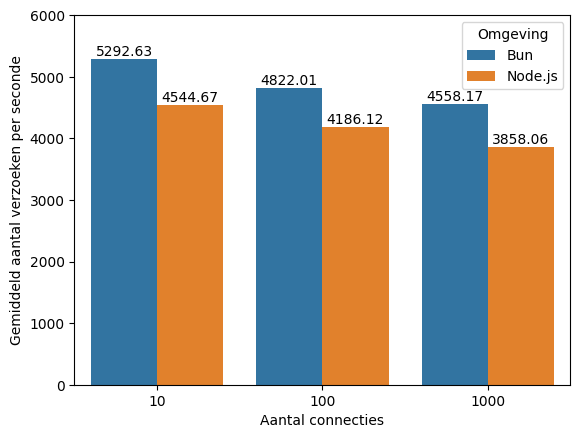
\includegraphics[width=0.7\columnwidth]{graphics/PostPostgresVerzoeken.png}
    \caption{\label{fig:postaantalverzoekenpostgres}Visuele voorstelling gemiddeld aantal verzoeken per seconde bij het maken van een recensie.}
  \end{figure}
  \begin{figure}[H]
    \centering
    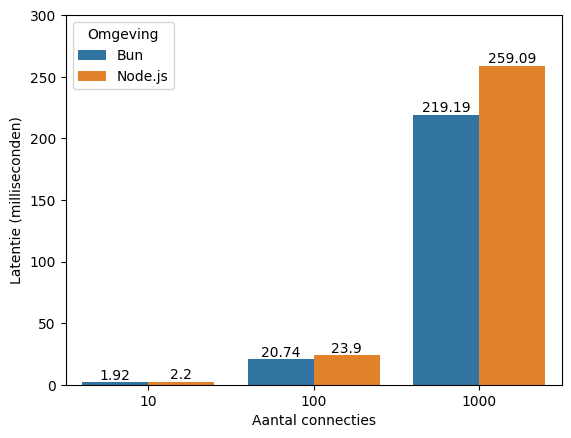
\includegraphics[width=0.7\columnwidth]{graphics/PostPostgresLatentie.png}
    \caption{\label{fig:postaantallatentiepostgres}Visuele voorstelling gemiddelde latentie bij het maken van een recensie.}
  \end{figure}
  \begin{figure}[H]
    \centering
    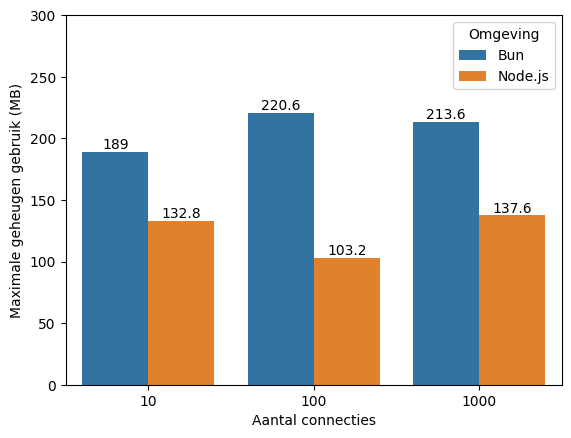
\includegraphics[width=0.7\columnwidth]{graphics/PostPostgresRAM.png}
    \caption{\label{fig:postgeheugenpostgres}Visuele voorstelling maximale geheugen gebruik bij het maken van een recensie.}
  \end{figure}
  \begin{figure}[H]
    \centering
    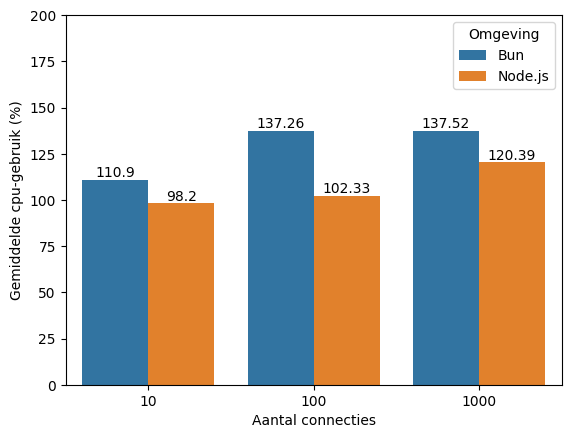
\includegraphics[width=0.7\columnwidth]{graphics/PostMySqlCpu.png}
    \caption{\label{fig:postcpupostgres}Visuele voorstelling gemiddeld CPU-gebruik bij het maken van een recensie.}
  \end{figure}
\subsection{Discussie}
Aan de hand van de Quick Sort algoritme resultaten kan het standpunt dat Bun computationeel sneller is ondersteund worden.
Zo was de gemiddelde uitvoeringstijd van Bun gemiddeld 2.21 keer sneller dan Node.js en lag het middelengebruik bij Bun ook lager. Deze snellere uitvoeringstijd komt door de
het gebruik van de JavaScriptScore engine in Bun waarbij geoptimaliseerde machine code wordt geproduceerd in 
samenwerking met 3 JIT compilers en een Low-Level interpreter.
Deze snelheid is niet enkel zichtbaar bij het algoritme, maar ook bij de installatietijd van de packages.
Zo is Bun met een gemiddelde installatietijd van 24,9 milliseconden 24,5 keer sneller is dan Node.js met een 
gemiddelde installatietijd van 610,1 milleseconden. Dit kan een groot verschil betekenen op vlak van efficiëntie in projecten 
met een groot aantal packages.
Met behulp van de recensie applicatie kan er ook gekeken worden naar de performantie bij I/O-taken.
In de metingen werd hiervoor een GET en POST endpoint opengezet waarbij telkens met een MySQL database en een PostgreSQL database de metingen werden uitgevoerd.
Bij het ophalen van data scoort Bun bij zowel de MySQL database als de PostgreSQL database telkens beter dan Node.js op vlak van het gemiddeld aantal verzoeken per seconde en de latentie.
Het verschil in aantal verzoeken per seconde toont aan dat Bun een grotere capaciteit voor verzoeken heeft bij het ophalen van data.
De latentie toont aan dat Bun sneller de opgehaalde data kan teruggeven. Echter komen deze voordelen met een prijs. 
Zo heeft Bun telkens een groter gebruik van middelen tegenover Node.js wat aantoont dat Node.js efficiënter is op vlak van geheugen management en CPU-management.
Bij het invoegen van data was er een gelijkaardige situatie. 
Bij de MySQL databank presteert Bun beter dan Node.js op zowel het vlak van het gemiddeld aantal verzoeken als de latentie bij 50 en 100 connecties. 
Echter zet dit zich niet voort in het middelengebruik waarbij Bun telkens weer meer middelen gebruikt als Node.js.
Bij de PostgreSQL database scoort Bun beter bij 10,50 en 100 connecties op vlak van latentie en verzoeken 
per seconde maar verbruikt het ook weer meer middelen om deze resultaten te bekomen. 
Op basis van deze bevindingen kunnen verschillende conclusies worden getrokken. 
Zo kunnen applicaties met complexe algoritmes en calculaties beter kiezen voor Bun. 
Deze kan doormiddel van zijn geoptimaliseerde machine code de calculaties sneller uitvoeren dan Node.js.
Bij I/O-taken moet er echter een afweging gemaakt worden. Zo is Bun in samenwerking met een PostgreSQL database sneller voor het ophalen en invoegen van data.
Echter komt dit ten koste van een hoger middelengebruik op vlak van geheugen en CPU. 
Indien de server hardware over voldoende middelen beschikt kan Bun gebruikt worden voor een snellere verwerking van de applicatie.


% Voeg hier je eigen hoofdstukken toe die de ``corpus'' van je bachelorproef
% vormen. De structuur en titels hangen af van je eigen onderzoek. Je kan bv.
% elke fase in je onderzoek in een apart hoofdstuk bespreken.

%\input{...}
%\input{...}
%...

%%=============================================================================
%% Conclusie
%%=============================================================================

\chapter{Conclusie}%
\label{ch:conclusie}

% TODO: Trek een duidelijke conclusie, in de vorm van een antwoord op de
% onderzoeksvra(a)g(en). Wat was jouw bijdrage aan het onderzoeksdomein en
% hoe biedt dit meerwaarde aan het vakgebied/doelgroep? 
% Reflecteer kritisch over het resultaat. In Engelse teksten wordt deze sectie
% ``Discussion'' genoemd. Had je deze uitkomst verwacht? Zijn er zaken die nog
% niet duidelijk zijn?
% Heeft het onderzoek geleid tot nieuwe vragen die uitnodigen tot verder 
%onderzoek?

In dit onderzoek werd aan de hand van een selectie gekozen om de performantie van Bun te vergelijken met Node.js om zo een antwoord te vinden op de 
onderzoeksvraag of Bun een correcte plaatsvervanger is van Node.js binnen de ontwikkeling van performante JavaScript applicaties.
In deze selectie werden de omgevingen afgetoetst aan een lijst van voorgedefinieerde requirements. Hierbij voldeed enkel Bun aan alle requirements.
Om deze onderzoeksvraag te kunnen beantwoorden werd aan de hand van de literatuurstudie en proof-of-concept een antwoord gezocht op volgende deelvragen:
\begin{itemize}
    \item Wat zijn de onderliggende verschillen tussen Node.js en Bun?
    \item Is Bun performanter dan Node.js bij het uitvoeren van logische berekeningen?
    \item Is Bun performanter dan Node.js bij het afhandelen van netwerk verzoeken?
    \item Wat is het verschil tussen hun respectievelijke package managers?
  \end{itemize}

De deelvraag betreffende de onderliggende verschillen werd beantwoord door middel van de literatuurstudie.
Hierbij werd uitgelegd dat Bun een andere JavaScript engine gebruikt dan Node.js om zo onder andere een snellere opstarttijd te bereiken.
Zo gebruikt Bun de JavaScriptCore engine in plaats van de V8 JavaScript engine die Node.js gebruikt.
Deze engine kan geoptimaliseerde machine code produceren in samenwerking met 3 JIT compilers en een Low-Level interpreter.
Daarnaast wordt ook een andere programmeertaal gebruik bij beide omgevingen. Zo wordt C gebruikt bij Node.js, terwijl Bij Bun werd gekozen voor Zig.
Tot slot heeft Bun veel zaken ingebouwd die bij Node.js extra moeten worden toegevoegd.
Het gaat hierbij over:
\begin{itemize}
    \item Een ingebouwde Test runner.
    \item Een ingebouwde bundler.
    \item Standaard TypeScript ondersteuning.
\end{itemize}
Uit de metingen van de proof-of-concepts kon een antwoord gevonden worden op de overige 3 deelvragen.
Hierbij werd voor zowel Bun als Node.js telkens 2 proof-of-concepts opgezet. 
Eén van deze proof-of-concept bestond uit een script dat het Quick Sort algoritme uitvoert om zo de performantie van logische berekeningen te meten.
Daarnaast werd voor de performantie bij netwerk verzoeken te meten een applicatie backend opgesteld. Met deze applicatie kunnen gebruikers
een lijst van onderwerpen ophalen en zelf recensies schrijven over een van deze onderwerpen.
Bij deze backend wordt het Sequelize ORM gebruikt in combinatie met zowel een MySQL databank als een PostgreSQL databank.
Uit de resultaten van het Quick Sort algoritme bleek dat Bun performanter is bij het uitvoeren van logische berekeningen.
Zo had Bun een gemiddelde uitvoeringstijd die 2,21 keer sneller was dan Node.js.
Bij het ophalen van data was er ook een groot performantie verschil tussen beiden. Zo had Bun met zowel de MySQL database als de PostgreSQL database 
een beter gemiddelde op vlak van aantal verzoeken per seconde en latentie. Echter bereikte Bun dit door een hoger gebruik van CPU- en geheugenmiddelen.
Bij het invoegen van data scoorde Bun beter dan Node.js op vlak van gemiddeld aantal verzoeken en latentie.
Enkel bij 10 connecties met een MySQL databank was Bun gelijkaardig aan Node.js.
Echter gebruikte Bun telkens meer middelen dan Node.js.
Uit deze resultaten kan geconcludeerd worden dat Bun algemeen sneller netwerk verzoeken kan afhandelen
ten koste van een hoger middelengebruik.
Als laatste werd ook de installatietijd onderzocht bij de package managers. Hierbij had Bun een 
gemiddelde installatietijd van 24,9 milliseconden, wat 24,5 keer sneller was dan Node.js, met een gemiddelde installatietijd van 610,1 milliseconden.
Dit toont een significant verschil tussen de respectievelijke package managers waarbij Bun beter presteert.

Het onderzoek geeft een leidraad bij de keuze van een JavaScript runtime-omgeving.
Zo blijkt uit de metingen Bun een optimale keuze te zijn voor applicaties met complexe algoritmes en calculaties door zijn geoptimaliseerde machine code.
Echter moet bij applicaties waarbij I/O-taken worden uitgevoerd telkens een afweging worden gemaakt tussen de snellere verwerking van Bun en het hogere middelengebruik dat dit teweeg brengt.


Voor de metingen werden uitgevoerd, was er de verwachting dat Bun beter ging presteren op basis van eerder uitgevoerd onderzoek vanuit de literatuurstudie en de selectie.
Op vlak van logische berekeningen en package managers zit dit in lijn met de bekomen resultaten, echter spreken de resultaten bij de server de verwachte conclusie enigszins tegen.
Zo presteert Bun wel beter bij het verwerken van verzoeken maar scoort het slechter op vlak van middelengebruik wat ook onderdeel uitmaakt van de performantie van een omgeving.
Bij 10 connecties in combinatie met een MySQL databank presteert Bun bij het invoegen van data zelfs vergelijkbaar met Node.js, 
terwijl het wel een hoger gebruik van middelen heeft.
Dit verschil ten opzichte van de verwachtingen kan te maken hebben met het feit dat eerdere onderzoeken alleen op kleine schaal werden uitgevoerd zonder ORM of databanken.

Toekomstig onderzoek kan verder gaan op de bekomen resultaten door in plaats van relationele databanken, zoals MySQL en PostgreSQL, ook NoSQL databases te testen.
Daarnaast zou ook de test runner en bundler van Bun kunnen vergeleken worden met andere alternatieven.



%---------- Bijlagen -----------------------------------------------------------

\appendix

\chapter{Onderzoeksvoorstel}

Het onderwerp van deze bachelorproef is gebaseerd op een onderzoeksvoorstel dat vooraf werd beoordeeld door de promotor. Dat voorstel is opgenomen in deze bijlage.

%% TODO: 
\section*{Samenvatting}
In de voorbije jaren zijn er voortdurend nieuwe javascript runtime-omgevingen ontwikkeld met telkens nieuwe verbeteringen. 
Echter worden weinig van deze nieuwe ontwikkelingen effectief in de praktijk gebruikt.
Zo is het oudere Node.js nog altijd de standaard in de industrie. 
In dit onderzoek wordt bestudeerd of deze nieuwere frameworks een meerwaarde bieden op vlak van performantie.
De onderzoeksvraag hierbij is of één van deze nieuwe frameworks  
een correcte plaatsvervanger kan zijn voor Node.js bij de ontwikkeling van webapplicaties binnen bedrijven 
waar performantie centraal staat.
Hiervoor werd voor beide frameworks een proof-of-concept gemaakt waarop performantie testen werden uitgevoerd.
Doormiddel van de testresultaten kon de performantie tussen de twee frameworks worden vergeleken.
Daarnaast werden ook een vergelijking tussen hun respectievelijke package managers uitgewerkt. 
Het resultaat zijn verschillende metingen van beide frameworks die kunnen worden vergeleken.
Er wordt hierbij verwacht dat het nieuwe framework Bun beter presteert dan Node.js door zijn focus op performantie.
Op basis van deze vergelijking kan een onderbouwde keuze worden gemaakt bij de selectie van een javascript runtime-omgeving.
% Kopieer en plak hier de samenvatting (abstract) van je onderzoeksvoorstel.

% Verwijzing naar het bestand met de inhoud van het onderzoeksvoorstel
%---------- Inleiding ---------------------------------------------------------

\section{Introductie}%
\label{sec:introductie}
In de afgelopen jaren zijn er heel wat nieuwe javascript runtime-omgevingen geïntroduceerd. 
Echter worden weinig van deze nieuwe environments effectief gebruikt. 
Zo toont onderzoek van ~\textcite{Greif2022} aan dat 93.6\% van de 29888 bevraagden Node.js regulier gebruiken.
Dit tegenover de 11.2\% en 4.3\% van de mensen die respectievelijk Deno en Bun geregeld gebruiken.
Momenteel wordt Node.JS nog altijd als standaard gebruikt bij elk project. 
Er zijn echter nog tal van andere javascript runtime-omgevingen, zoals bovengenoemde Bun en Deno, 
die in staat zijn om specifieke noden te vervullen waar Node.js niet kan aan voldoen.
Het doel van deze studie is te onderzoeken of één van deze nieuwe frameworks een correcte plaatsvervanger kan zijn voor Node.js
bij de ontwikkeling van webapplicaties binnen bedrijven zoals Codifly waar performantie centraal staat. Hierbij spelen verschillende aspecten een rol.
Is het nieuwe framework performanter? Wat is het verschil tussen de package managers?
Hoe complex is het nieuwe framework tegenover Node.js?
Om deze vragen te beantwoorden wordt de 
performantie en complexiteit tussen Node.js en het nieuwe framework Bun vergeleken aan de hand van een proof-of-concept.
Hierbij wordt de performantie zowel gemeten bij simpele applicaties zoals het uitvoeren van logische berekeningen
als meer complexe applicaties waarbij netwerk verzoeken worden gebruikt.
In wat volgt wordt eerst een overzicht gegeven van de actuele ontwikkelingen binnen het
onderzoeksdomein aan de hand van een literatuurstudie, waarna de methodologie wordt besproken.
Ten laatste worden de resultaten van de vergelijking alsook de conclusie besproken.


%---------- Stand van zaken ---------------------------------------------------

\section{State-of-the-art}%
\label{sec:state-of-the-art}
% Voor literatuurverwijzingen zijn er twee belangrijke commando's:
% \autocite{KEY} => (Auteur, jaartal) Gebruik dit als de naam van de auteur
%   geen onderdeel is van de zin.
% \textcite{KEY} => Auteur (jaartal)  Gebruik dit als de auteursnaam wel een
%   functie heeft in de zin (bv. ``Uit onderzoek door Doll & Hill (1954) bleek
%   ...'')
Javascript vormt de basis voor alle Javascript runtime-omgevingen. 
Het is een geïnterpreteerde programmeertaal dat vooral bekend is bij front-end web development voor web pagina's ~\autocite{Mozilla2023}.
Echter kan het ook buiten browser omgevingen gebruikt worden met behulp van javascript runtime-omgevingen zoals Node.js,Bun en Deno ~\autocite{Mozilla2023}.
Zo een omgeving bestaat uit alle componenten om javascript correct te laten werken ~\autocite{Christopher}. 
Het bevat een JavaScript engine, WEB API's en een callback queue ~\autocite{Christopher}. 
Deze runtime zal dan javascript code omzetten in code die verstaanbaar is voor de computer.
De omgeving specificeert waar dit wordt gedaan, dit kan in een browser maar ook in andere omgevingen.
De afgelopen jaren is het aantal van deze soort omgevingen sterk toegenomen. 
De meest bekende en oudste is Node.js. 
Node.js is een server-side framework dat wordt gebruikt voor schaalbare applicaties te maken ~\autocite{Gackenheimer2013}.
In het boek van ~\textcite{Ali2013} wordt verteld hoe Node.js zich onderscheidt van andere platformen door het gebruik van een event loop. 
Wanneer in Node.js een I/O operatie wordt verwerkt zal een gebeurtenis worden uitgezonden. 
De event loop zal continu kijken of er zo gebeurtenissen voorkomen, 
en wanneer dit zo is zal het deze plaatsen in de event wachtrij. 
De event loop zal dan deze wachtrij doorgaan en één per één de event handlers uitvoeren. 
Dit laat toe om I/O operaties asynchroon te maken.
De JavaScript code binnenin Node.js wordt uitgevoerd door de V8 JavaScript engine, 
dezelfde engine die toelaat om JavaScript uit te voeren in Chrome ~\autocite{Syed2014}.
Hierbij wordt gebruikgemaakt van een call stack en een heap. 
De call stack is de plaats waar de code wordt uitgevoerd,terwijl de heap de plaats is waar alle nodige objecten worden opgeslagen ~\autocite{Christopher}.
Doordat JavaScript files steeds groter werden, werd in 2009 CommonJS geïntroduceerd. 
Dit specificeert een simpele API om modules te declareren die werken buiten de browser ~\autocite{Osmani2012}.
Hierbij is een module een stuk herbruikbare code dat kan gebruikt worden in  andere code ~\autocite{Osmani2012}.
Node.js volgt de CommonJS module specificatie, waarbij elk bestand zijn eigen module vormt ~\autocite{Syed2014}.
Buiten zelf modules te schrijven, bestaan er ook modules die geschreven zijn door andere mensen. 
Deze zijn te vinden in de Node Package Manager (NPM) ~\autocite{Wittern2016}. 
Deze modules kunnen dan gebruikt worden door andere mensen in hun eigen project ~\autocite{Ali2013}.

Performantie is één van de belangrijkste zaken bij een server-side framework. Daarom is Node.js dankzij zijn 
event-gedreven I/O model een veelvoorkomende keuze als het gaat om server-side frameworks. 
Echter wil Bun dit veranderen door nog meer focus te leggen op snelheid en performantie. 
Om dit te bereiken maakt Bun gebruik van JavaScriptCore in plaats van de V8 JavaScript engine ~\autocite{McDonnel2023}.
Dit is de ingebouwde engine voor WebKit, een web browser engine die wordt gebruikt op macOS en IOS ~\autocite{Pizlo2020}.
Door het gebruik van de JavaScriptCore engine zou Bun 4 keer sneller kunnen opstarten dan Node.js ~\autocite{McDonnel2023}.
Bun bevat daarnaast ook een test runner,script runner en een Node.js compatibele package manager, die volgens ~\textcite{McDonnel2023} 
allemaal significant sneller zijn dan bestaande applicaties zoals Node.js en Deno.
Een ander verschil tussen Node.js en Bun is de ingebouwde support voor TypeScript en JSX. 
Terwijl bij Node.js je hiervoor aparte packages nodig hebt, 
zal bij Bun de transpiler deze bestanden automatisch converteren naar vanilla Javascript.

Doordat Bun redelijk nieuw is, zijn er nog maar weinig onderzoeken over gedaan.
Eén van deze onderzoeken werd uitgevoerd door ~\textcite{Feroj2023}.
Hierbij werd de performantie tussen Node.js en Bun vergeleken op basis van verschillende performantie attributen. 
Deze omvatten geheugengebruik, antwoordtijd en de algemene uitvoeringstijd. 
Voor het testen van netwerk verzoeken werd bij beiden gebruikgemaakt van Bombardier. Hierbij werden in 3 aparte scenario's, 
10 miljoen verzoeken gemaakt met eerst 10 gelijktijdige connecties, dan 100 gelijktijdige connecties en
uiteindelijk 500 gelijktijdige connecties. Hierbij kon de onderzoeker de performantie van de servers evalueren 
aan de hand van responstijd en doorvoer. Aanvullend werden ook de geheugengebruik pieken bepaald.
Daarnaast werd ook getest hoe beide runtimes een alleenstaand script afhandelen. 
Dit werd gedaan aan de hand van Hyperfine, een command-line process benchmark hulpmiddel. 
Hierbij werd de executie tijd gemeten in zowel Bun als Node.js voor het berekenen van Fibonacci nummers.
Het eerste resultaat toont het verschil in geheugengebruik tussen Bun en Node.js. 
Hierbij heeft Bun consistent een lager geheugengebruik tegenover Node.js en toont het aan dat Bun een beter geheugenbeheer heeft.
De onderzoeker merkt op dat de oorzaak hiervan ligt bij Bun's gebruik van Zig, 
een programmeertaal gekend voor zijn effectiviteit en geheugenbeheer. 
Ook op vlak van executie tijd, responstijd en doorvoer presteerde Bun consistent beter dan Node.js. 
Deze resultaten tonen aan dat Bun algemeen beter presteert in zowel het afhandelen van netwerk verzoeken 
als het uitvoeren van computationele taken.
De onderzoeker merkt echter ook op dat de keuze van een runtime niet alleen kan bepaald worden op basis van performantie. 
Andere factoren, die hier niet getest zijn, zoals beveiling, stabiliteit en onderhoudbaarheid dragen ook bij tot de keuze. 
Ook waren de geteste programma's redelijk simpel waardoor de resultaten mogelijks niet accuraat zijn voor complexere omgevingen.
Verder onderzoek zou ook baat hebben om rekening te houden met verschillende omstandigheden, 
zoals CPU-gebonden en I/O-gebonden processen.

Een ander nieuw framework is Deno. 
Dit framework werd geïntroduceerd door ~\textcite{Dahl2021}, de maker van Node.js.
Met Deno wil hij nieuw leven inblazen in het ecosysteem door middel van een modern, productief programmeer systeem aan te bieden dat zich houdt aan browser API's.
Net zoals Node.js gebruikt Deno de V8 Javascript engine ~\autocite{DenoLand2023}. Echter werd Deno ontwikkeld in Rust, terwijl Node in C en C++ ~\autocite{DenoLand2023}. 
Eén van de kenmerken van Deno is de beveiliging. Zo is er standaard runtime-beveiliging, 
waarbij je als ontwikkelaar expliciet moet toestaan dat code toegang mag krijgen tot gevoelige API's ~\autocite{DenoLand2023}.
Technisch gezien heeft Deno geen package manager. Het maakt gebruik van URL's om externe modules te importeren ~\autocite{DenoLand2023}.
Het voordeel hierbij is dat wanneer je een module importeert, deze automatisch wordt gecached ~\autocite{DenoLand2023}.

Doordat Deno redelijk recent, zijn er ook hier nog maar weinig onderzoeken over gedaan.
Eén van deze onderzoeken werd uitgevoerd door ~\textcite{VanKerkvoorde2021}. 
Hierbij werd Node.js vergeleken met Deno op verschillende vlakken zoals performantie en beveiliging.
Op vlak van beveiliging scoort Deno beter dan Node.js door middel van standaard geen toegang te geven tot de folderstructuur en omgeving. 
Ook kunnen er standaard geen netwerk connecties worden gemaakt. 
Voor de performantie te testen van beide frameworks werd allereerst een logica test uitgevoerd op beiden. 
De onderzoeker heeft hierbij ondervonden dat Deno gemiddeld 31.98\% sneller was dan Node.js. Ook gebruikte Node hier 10.81 keer meer geheugen.
Als tweede test werden de Http modules van beide frameworks vergeleken. Hiervoor werd een simpele GET request verstuurd naar beiden. 
Hierbij was er geen significant verschil tussen beiden volgens de onderzoeker.
Echter heeft de onderzoeker voor beide frameworks ook een concrete backend geschreven. Voor Node.js werd hierbij Express gebruikt terwijl bij Deno Oak.
Hierbij werd er wel een groot verschil waargenomen tussen de 2 frameworks, waarbij Deno performanter was dan Node.
Volgens de onderzoeker blijkt uit de testen dat Deno beter scoort dan Node op vlak van verwerkingstijd en geheugengebruiker.
De onderzoeker merkt wel op dat door het gebrek aan bepaalde metrieken binnen Deno, zaken zoals CPU- en GPU-belasting niet konden worden gemeten.
%---------- Methodologie ------------------------------------------------------
\section{Methodologie}%
\label{sec:methodologie}
Het onderzoek bevat 7 fasen.
De eerste fase is een algemene beschrijving van Node.js alsook een beschrijving van de mogelijke alternatieven. 
Dit wordt gedaan aan de hand van een literatuurstudie van wetenschappelijke artikels en boeken. 
De geschatte duurtijd van dit proces is 2 weken.

De tweede fase bestaat uit het verzamelen van de criteria die zal getest worden bij beide omgevingen. 
De focus ligt hierbij op performantie en complexiteit.
Dit gebeurt in samenspraak met de co-promotor. Hierbij worden deze criteria geordend volgens belang. 
De verzameling van deze criteria duurt 1 week.

In de derde fase wordt een long list opgesteld met mogelijke alternatieven voor Node.js. 
Deze worden geanalyseerd aan de hand van een literatuuronderzoek. Deze analyse bedraagt 1 week en loopt samen met het verzamelen van de criteria.

De vierde fase bestaat uit het selecteren van één framework uit de long list die het beste voldoet aan de vereisten. 
Dit proces zal 1 week in beslag nemen.

In de vijfde fase zal een zelfgemaakte proof-of-concept ontworpen worden voor zowel Node.js als het geselecteerde framework. 
Hierbij wordt een applicatie ontwikkeld waarbij een gebruiker een recensie kan creëren over een bepaald onderwerp, 
alsook een script dat een algoritme bevat.
Voor deze ontwikkeling is een geschatte duurtijd van 3 weken voorzien.

In de zesde fase worden te testen uitgevoerd op de proof-of-concepts. 
Hierbij zal gebruik gemaakt worden van benchmark tools Hyperfine en Bombardier om de responstijd, installatietijd en uitvoeringstijd te testen.
Voor het visualiseren van de metingen zal Seaborn worden gebruikt.
Dit proces neemt 4 weken in beslag.

De laatste fase bevat een conclusie over de vergelijking. 
Hierbij wordt een aanbeveling gegeven op basis van de metingen en testen.
Dit neemt 1 week in beslag
\begin{figure}[h]
    \centering
    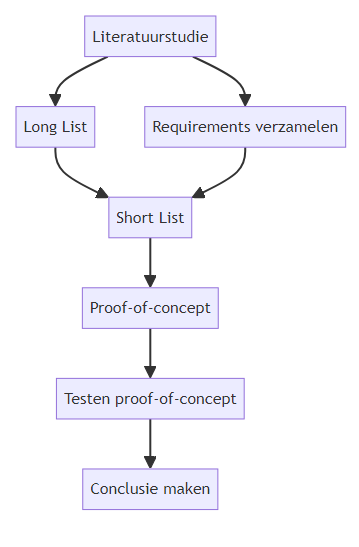
\includegraphics[width=.4\textwidth]{graphics/flowchart.png}
    \caption{\label{fig:flowchart}}Flowchart van methodologie
\end{figure}
%---------- Verwachte resultaten ----------------------------------------------
\section{Verwacht resultaat, conclusie}%
\label{sec:verwachte_resultaten}
Op basis van literatuuronderzoek zal gekozen worden om Bun te vergelijken met Node.js doordat dit framework zich focust op performantie.
De verwachte resultaten zijn metingen van de proof-of-concepts die aantonen dat Bun performanter is dan de Node.js (zie figuur~\ref{fig:uitvoeringstijd} en~\ref{fig:responstijd}). 
Deze metingen werden uitgevoerd met behulp van benchmark tools Hyperfine en Bombardier.
Ook wordt verwacht dat de package manager van Bun een snellere installatietijd heeft dan de Node Package Manager en dat Bun minder complex is dan Node.js (zie figuur~\ref{fig:installatietijd}).
Deze verwachtingen komen mede doordat Bun zich bij de ontwikkeling specifiek heeft gefocust op performantie-optimalisatie.
Ook heeft Bun redelijk wat zaken, zoals een test-runner, al ingebouwd wat het minder complex maakt dan Node.js.
Op basis van deze metingen kan een onderbouwde keuze worden gemaakt tussen het gebruik van Node.js en Bun bij de ontwikkeling
van performante webapplicaties.

Doordat Node.js nog altijd de norm is, zal het zeer veel tijd vragen tegen dat Bun deze effectief kan vervangen.
Het is toch belangrijk dat er nu een keuze kan gemaakt worden tussen javascript runtime-omgevingen bij de ontwikkeling van applicaties.

\begin{figure}
    \centering
    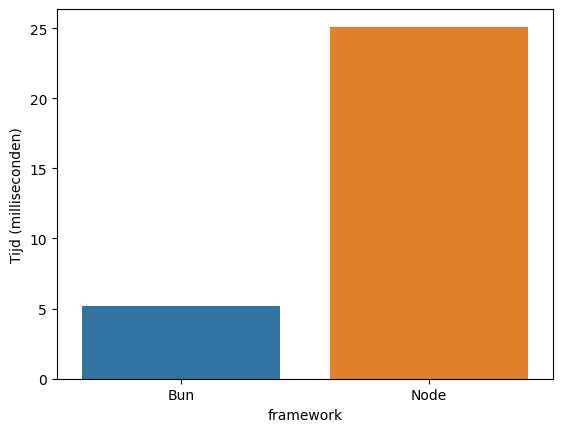
\includegraphics[width=.4\textwidth]{graphics/diagram.png}
    \caption{\label{fig:uitvoeringstijd}}Mock-up waarbij we zien dat Bun een betere uitvoeringstijd heeft dan Node.js bij de uitvoering van een simpel algoritme.
    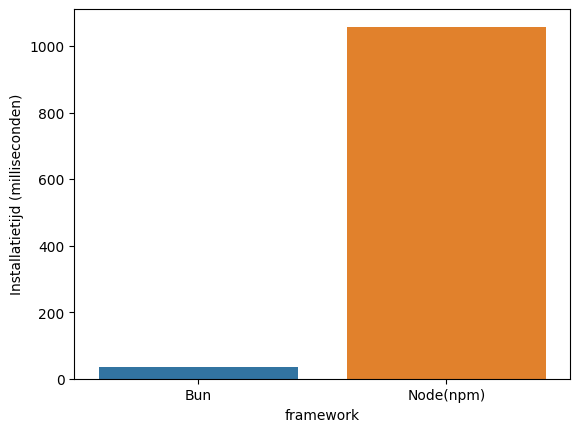
\includegraphics[width=.4\textwidth]{graphics/installatietijd.png}
    \caption{\label{fig:installatietijd}}Mock-up waarbij we zien dat Bun een betere installatietijd heeft dan Node.js bij het installeren van dependencies.
    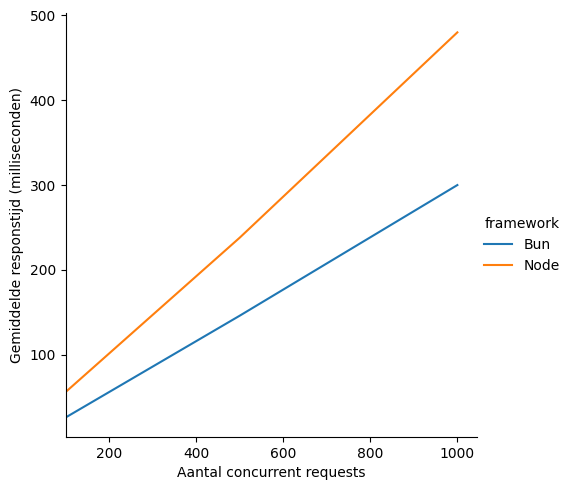
\includegraphics[width=.4\textwidth]{graphics/Responstijd.png}
    \caption{\label{fig:responstijd}}Mock-up waarbij we zien dat Bun een betere responstijd heeft dan Node.js bij het afhandelen van concurrent requests.
\end{figure}


%%---------- Andere bijlagen --------------------------------------------------
% TODO: Voeg hier eventuele andere bijlagen toe. Bv. als je deze BP voor de
% tweede keer indient, een overzicht van de verbeteringen t.o.v. het origineel.
%\input{...}

%%---------- Backmatter, referentielijst ---------------------------------------

\backmatter{}

\setlength\bibitemsep{2pt} %% Add Some space between the bibliograpy entries
\printbibliography[heading=bibintoc]

\end{document}
